\chapter{KESEHATAN KELUARGA}
Pembangunan keluarga dilakukan dalam upaya untuk mewujudkan keluarga berkualitas yang hidup dalam lingkungan yang sehat. Selain lingkungan yang sehat, kondisi kesehatan dari tiap anggota keluarga sendiri juga merupakan salah satu syarat dari keluarga yang berkualitas.
Keluarga berperan terhadap optimalisasi pertumbuhan, perkembangan, dan produktivitas seluruh anggotanya melalui pemenuhan kebutuhan gizi dan menjamin kesehatan anggota keluarga. 

Di dalam komponen keluarga, ibu dan anak merupakan kelompok rentan terhadap keadaan keluarga dan sekitarnya secara umum.
Hal ini terkait dengan fase kehamilan, persalinan dan nifas pada ibu dan fase tumbuh kembang pada anak.
Oleh karena itu ibu dan anak merupakan anggota keluarga yang perlu mendapatkan prioritas dalam penyelenggaraan upaya kesehatan.

\section{KESEHATAN IBU}
Seorang ibu mempunyai peranan yang sangat penting dalam pertumbuhan anak dan bayi.
Hal ini terkait dengan fase kehamilan, persalinan dan nifas pada ibu dan fase tumbuh kembang pada anak.
Gangguan kesehatan yang dialami pada seorang ibu dapat mempengaruhi kesehatan janin dalam kandungan hingga kelahiran dan masa pertumbuhan bayi dan anaknya.

\subsection{Angka Kematian Ibu (AKI)}
Kematian ibu adalah kematian yang terjadi pada seorang ibu yang terjadi karena peristiwa kehamilan, persalinan, dan masa nifas (dalam kurun waktu 42 hari sejak terminasi kehamilan) tanpa memandang lamanya kehamilan, yakni kematian yang disebabkan karena kehamilannya atau penanganannya, tetapi bukan karena sebab-sebab lain seperti kecelakaan dan terjatuh.
Angka Kematian Ibu (AKI) menggambarkan status gizi dan tingkat pelayanan kesehatan terhadap ibu hamil, ibu melahirkan dan ibu masa nifas.

Jumlah Kematian Ibu di Kabupaten Belitung Timur pada tahun \tP adalah 3 orang, dengan Angka Kematian Ibu (AKI) 157,48 per 100.000 kelahiran hidup (\autoref{fig:Jumlah-Kematian-Ibu}). 
%Angka ini meningkat dari AKI tahun 2020 sebesar 189,84 per 100.000 kelahiran hidup(\autoref{fig:AKI-2017-2021}).

\begin{figure}[H]
    \centering{}
    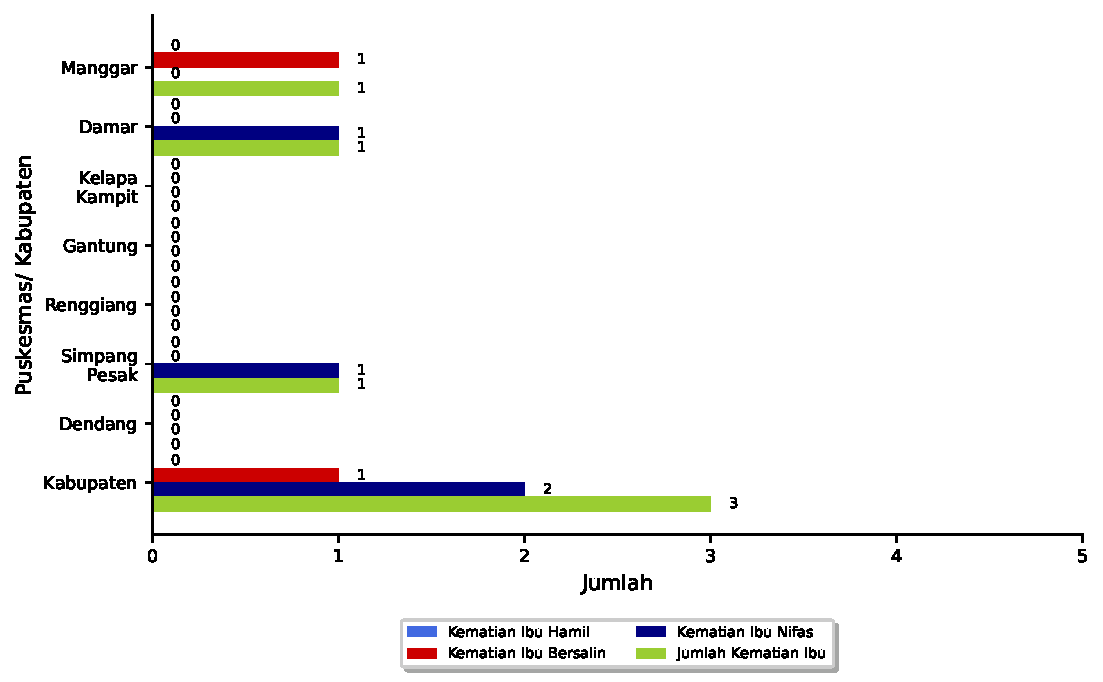
\includegraphics[width=0.9\textwidth]{bab_05/bab_05_01_kematianIbu}
%    \caption{Jumlah Kematian Ibu di Kab. Belitung Timur Tahun \tP per Puskesmas (hal. ~\pageref{C_21-Jumlah-Kematian-Ibu})}
    \caption{Jumlah Kematian Ibu di Kab. Belitung Timur Tahun \tP per Puskesmas}
    \label{fig:Jumlah-Kematian-Ibu}
\end{figure}

\begin{figure}[H]
    \centering{}
    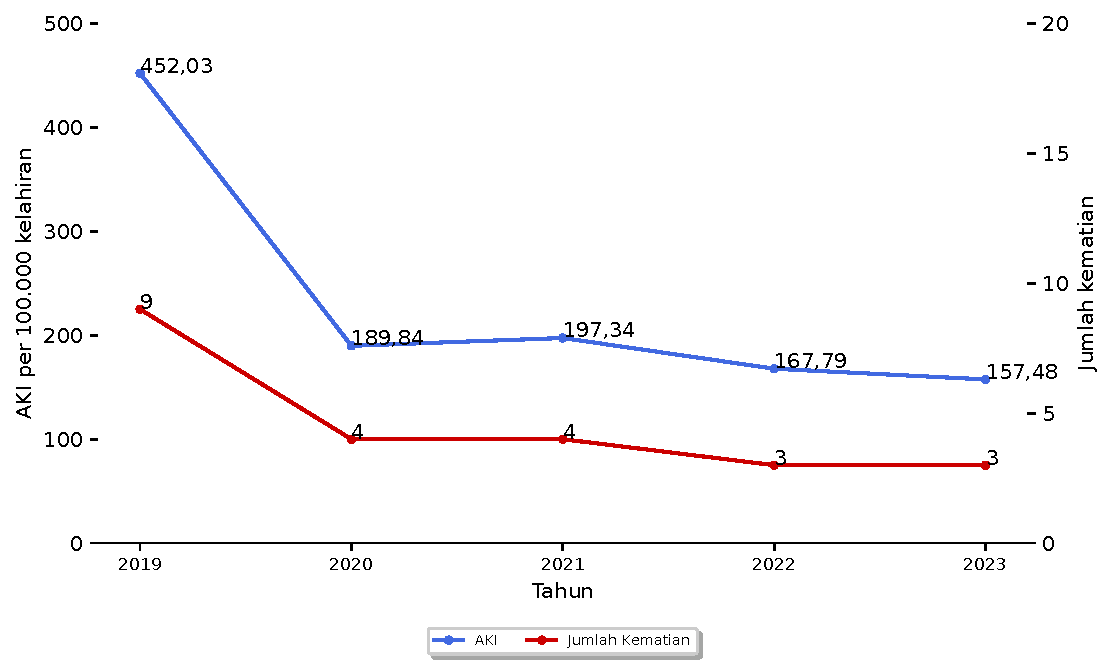
\includegraphics[width=0.85\textwidth]{bab_05/bab_05_02_plotAKI}
    \caption{AKI Kab. Belitung Timur 2019-2023}
    \label{fig:AKI-2019-2023}
\end{figure}

\subsection{Pelayanan Antenatal (K1, K4, dan K6)}
Cakupan kunjungan ibu hamil K-1 adalah cakupan kunjungan ibu hamil yang mendapat pelayanan antenatal sesuai standar (10T) oleh tenaga kesehatan pada masa kehamilan trimester
pertama di satu wilayah kerja pada kurun waktu tertentu. Cakupan ibu hamil K4 adalah cakupan ibu hamil yang mendapatkan pelayanan antenatal sesuai standar (10T) paling sedikit empat kali, dengan distribusi pemberian pelayanan yang dianjurkan adalah minimal satu kali pada trimester pertama, satu kali pada trimester kedua dan dua kali pada trimester ketiga umur kehamilan. Cakupan ibu hamil K6 adalah cakupan ibu hamil yang mendapatkan pelayanan antenatal sesuai standar (10T) paling sedikit enam kali, dengan distribusi pemberian pelayanan yang dianjurkan adalah minimal satu kali pada trimester pertama, dua kali pada trimester kedua dan tiga kali pada trimester ketiga dengan paling sedikit 2 kali oleh dokter pada trimester pertama dan ketiga.

Cakupan K1 dan K4 di Kabupaten Belitung Timur pada tahun \tP adalah sebesar 87,29\% dan 85,56\% (\autoref{fig:Cakupan-K1-K4}), meningkat dari cakupan tahun 2022 sebesar 86,27\% dan 81,52\%(\autoref{fig:Cakupan-K1-K4-2019-2023}).

\begin{figure}[H]
    \centering{}
    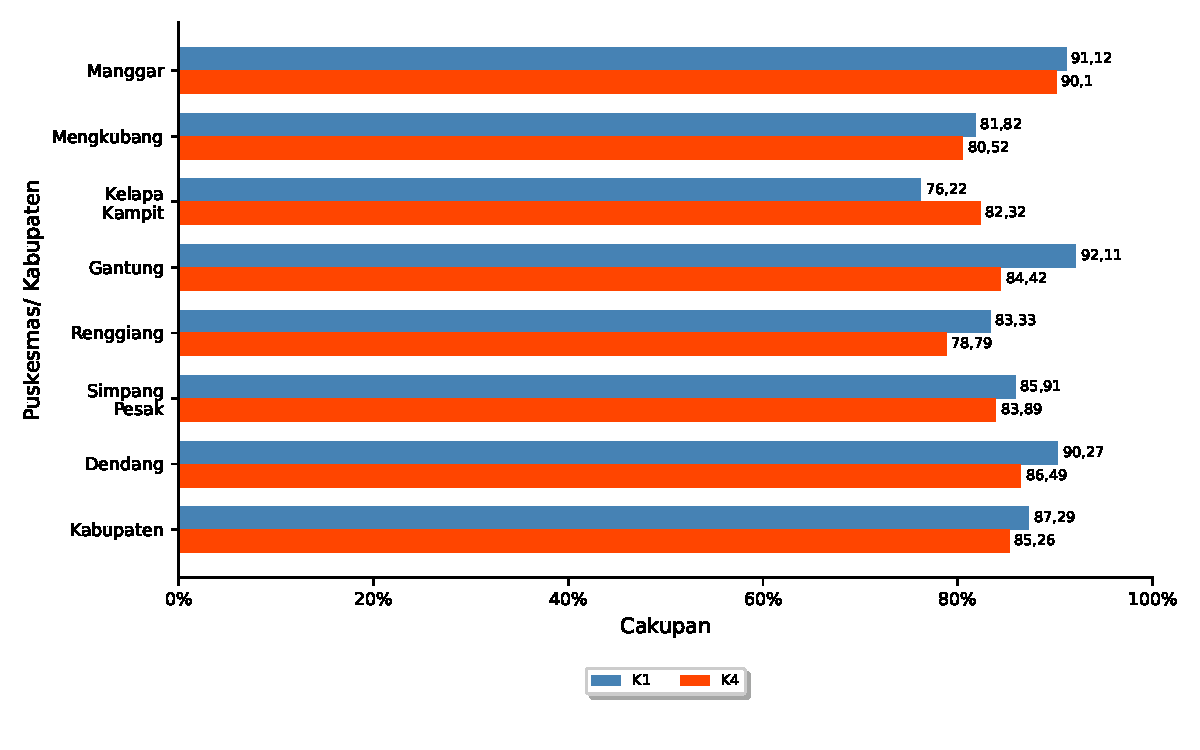
\includegraphics[width=0.9\textwidth]{bab_05/bab_05_03_K1K4}
    \caption{Cakupan K1 dan K4 di Kab. Belitung Timur Tahun \tP per Puskesmas}
    \label{fig:Cakupan-K1-K4}
\end{figure}

\begin{figure}[H]
    \centering{}
    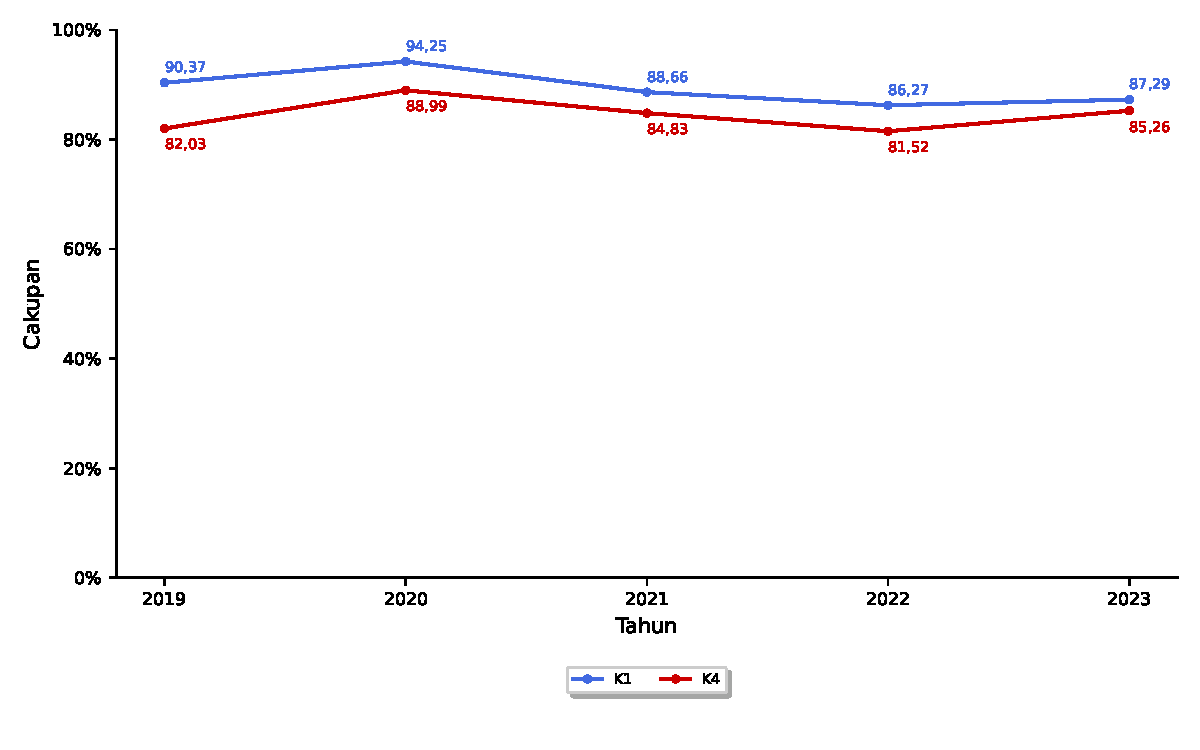
\includegraphics[width=0.85\textwidth]{bab_05/bab_05_03a_plotK1K4}
    \caption{Cakupan K1 dan K4 di Kab. Belitung Timur Tahun 2019-2023}
    \label{fig:Cakupan-K1-K4-2019-2023}
\end{figure}

Cakupan K6 di Kabupaten Belitung Timur pada tahun \tP adalah sebesar 83,37\% (\autoref{fig:Cakupan-K6}).

\begin{figure}[H]
	\centering{}
    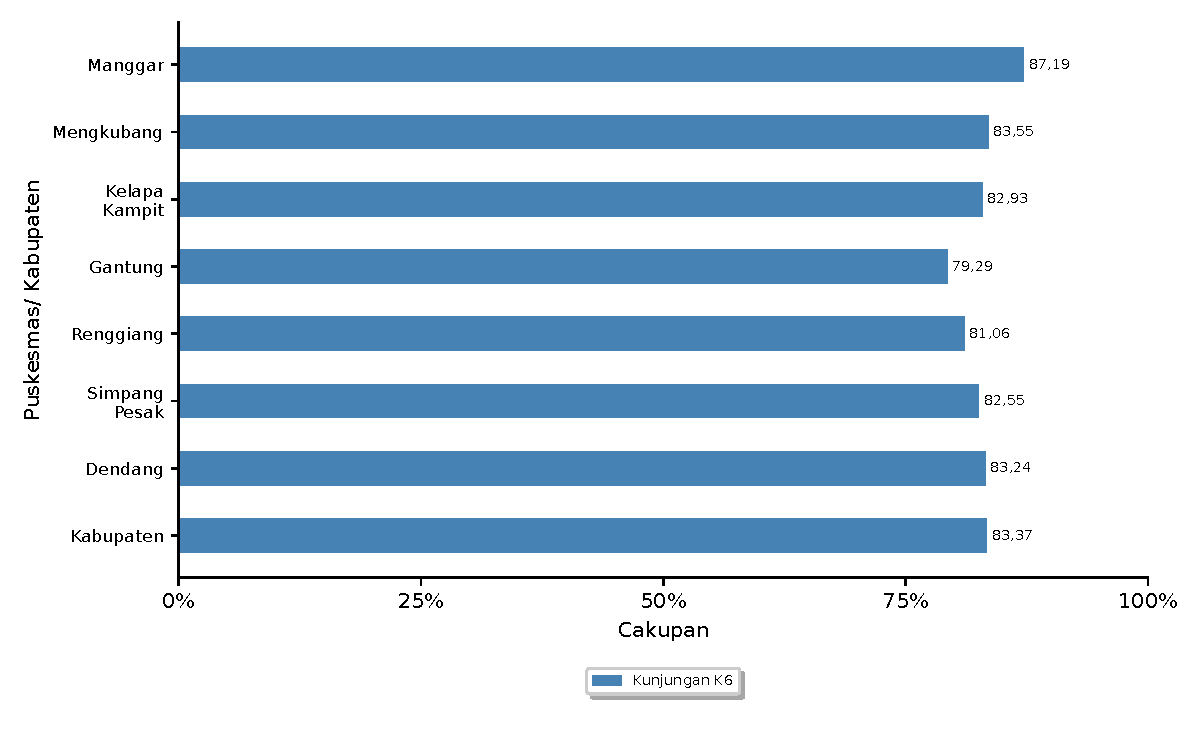
\includegraphics[width=0.9\textwidth]{bab_05/bab_05_03c_K6}
	\caption{Cakupan K6 di Kab. Belitung Timur Tahun \tP per Puskesmas}
	\label{fig:Cakupan-K6}
\end{figure}

\subsection{Imunisasi Td Ibu Hamil}
Peraturan Menteri Kesehatan Nomor 42 Tahun 2013 tentang Penyelenggaraan Imunisasi mengamanatkan bahwa wanita usia subur dan ibu hamil merupakan salah satu kelompok populasi yang menjadi sasaran imunisasi lanjutan.
Imunisasi lanjutan adalah kegiatan yang bertujuan untuk melengkapi imunisasi dasar pada bayi yang diberikan kepada anak batita, anak usia sekolah, dan wanita usia subur termasuk ibu hamil.
Salah satu upaya imunisasi lanjutan yang menyasar ibu hamil adalah imunisasi Td untuk mengendalikan infeksi tetanus yang merupakan salah satu faktor risiko kematian ibu dan kematian bayi.
Infeksi tetanus disebabkan oleh bakteri \emph{Clostridium tetani} sebagai akibat dari proses persalinan yang tidak aman/ steril atau berasal dari luka yang diperoleh ibu hamil sebelum melahirkan.

Cakupan Imunisasi Td pada ibu hamil adalah ang mendapatkan imunisasi Td (Tetanus difteri) dengan interval tertentu (yang dimulai saat dan atau sebelum kehamilan) dengan memperhatikan hasil skrining dan status T.

Cakupan Td5 ibu hamil di kabupaten Belitung Timur tahun \tP yaitu sebesar 74,49\%, sedangkan cakupan Td2+ yaitu sebesar 86,62\% (\autoref{fig:Cakupan-Td}).

\begin{figure}[H]
    \centering{}
    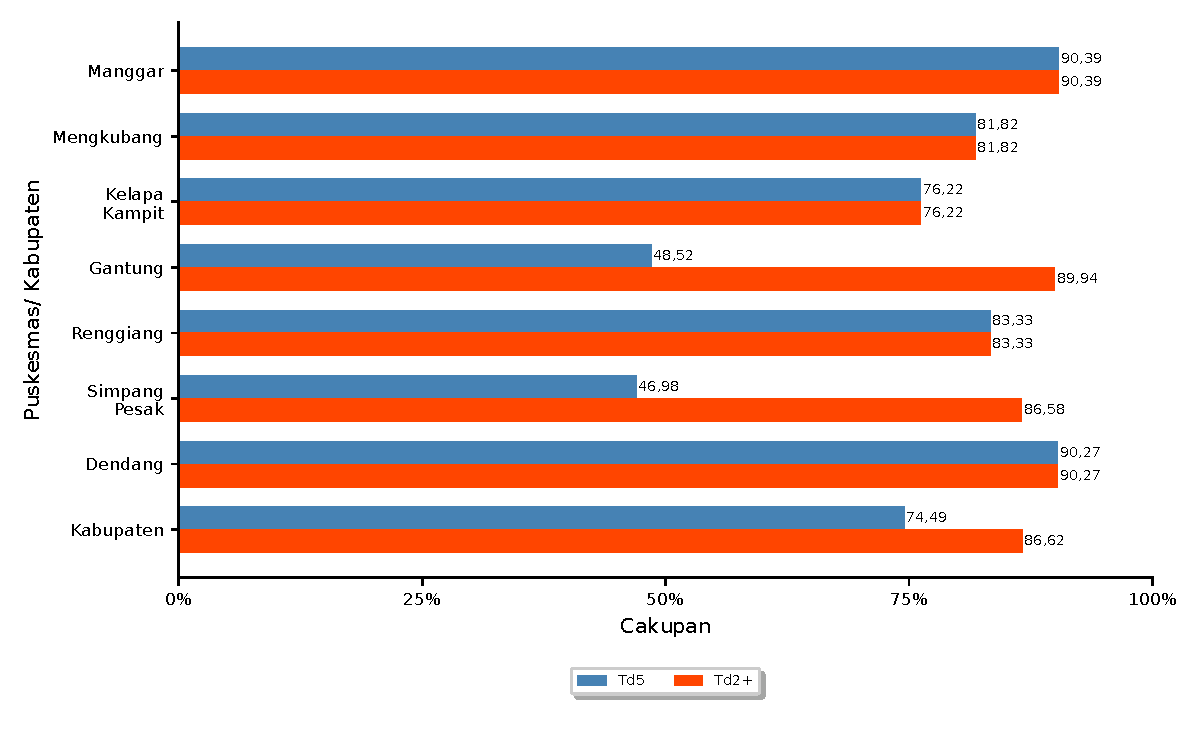
\includegraphics[width=0.85\textwidth]{bab_05/bab_05_04_Td}
    \caption{Cakupan Imunisasi Td Ibu Hamil di Kab. Belitung Timur Tahun \tP per Puskemas}
    \label{fig:Cakupan-Td}
\end{figure}

\subsection{Pemberian Tablet Tambah Darah}
Salah satu komponen pelayanan kesehatan ibu hamil yaitu pemberian suplemen zat besi sebanyak 90 tablet (Fe3).
Zat besi merupakan mineral yang dibutuhkan tubuh untuk membentuk sel darah merah (hemoglobin).
Zat besi memiliki peran vital terhadap pertumbuhan janin.
Selama hamil, asupan zat besi harus ditambah mengingat selama kehamilan, volume darah pada tubuh ibu meningkat.
Sehingga, untuk dapat tetap memenuhi kebutuhan ibu dan menyuplai makanan serta oksigen pada janin melalui plasenta, dibutuhkan asupan zat besi yang lebih banyak.

Cakupan ibu hamil mendapat TTD adalah persentase ibu hamil yang mendapatkan Tablet Tambah Darah (TTD) sekurangnya mengandung zat besi setara dengan 60 mg besi elemental dan 0,4 mg asam folat yang disediakan oleh pemerintah minimal 90 tablet selama masa kehamilan. Cakupan ibu hamil mengonsumsi TTD adalah persentase ibu hamil yang mengonsumsi Tablet Tambah Darah (TTD) sekurangnya mengandung zat besi setara dengan 60 mg besi elemental dan 0,4 mg asam folat yang disediakan oleh pemerintah minimal 90 tablet selama masa kehamilan.

Cakupan ibu hamil mendapat TTD di Kabupaten Belitung Timur pada tahun \tP adalah sebesar 82,02\% (\autoref{fig:Cakupan-TTD}).

\begin{figure}[H]
    \centering
    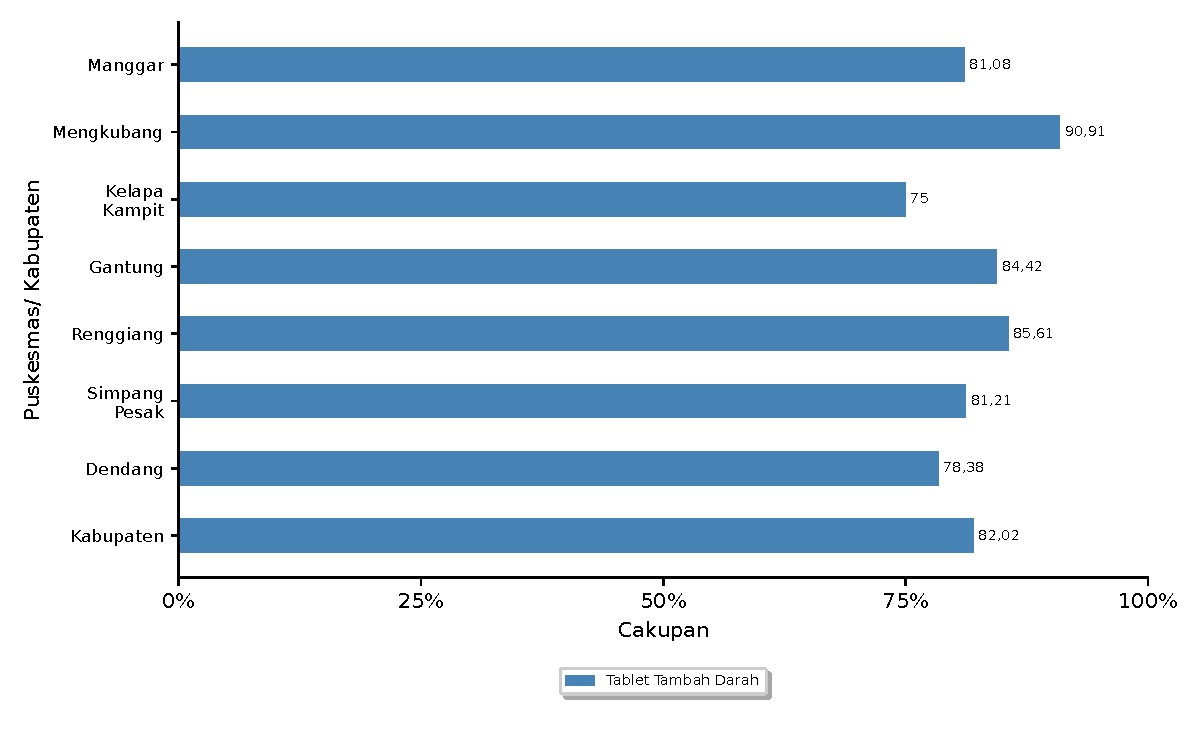
\includegraphics[width=0.9\textwidth]{bab_05/bab_05_05_TTD}
    \caption{Cakupan Pemberian TTD di Kab. Belitung Timur Tahun \tP per Puskesmas}
    \label{fig:Cakupan-TTD}
\end{figure}


\subsection{Pertolongan Persalinan oleh Tenaga Kesehatan dengan Kompetensi Kebidanan}
Salah satu upaya menekan angka kematian ibu dan bayi yaitu dengan mendorong upaya persalinan dilakukan oleh tenaga kesehatan dengan kompetensi kebidanan di fasilitas pelayanan kesehatan.

Cakupan persalinan di fasilitas pelayanan kesehatan adalah cakupan ibu bersalin yang mendapatkan pelayanan persalinan sesuai standar di fasilitas pelayanan kesehatan di satu wilayah kerja pada kurun waktu tertentu.

Cakupan persalinan di fasilitas pelayanan kesehatan di Kabupaten Belitung Timur pada tahun \tP yaitu sebesar 90,04\% (\autoref{fig:Cakupan-Persalinan-Fasyankes}).

\begin{figure}[H]
    \centering
    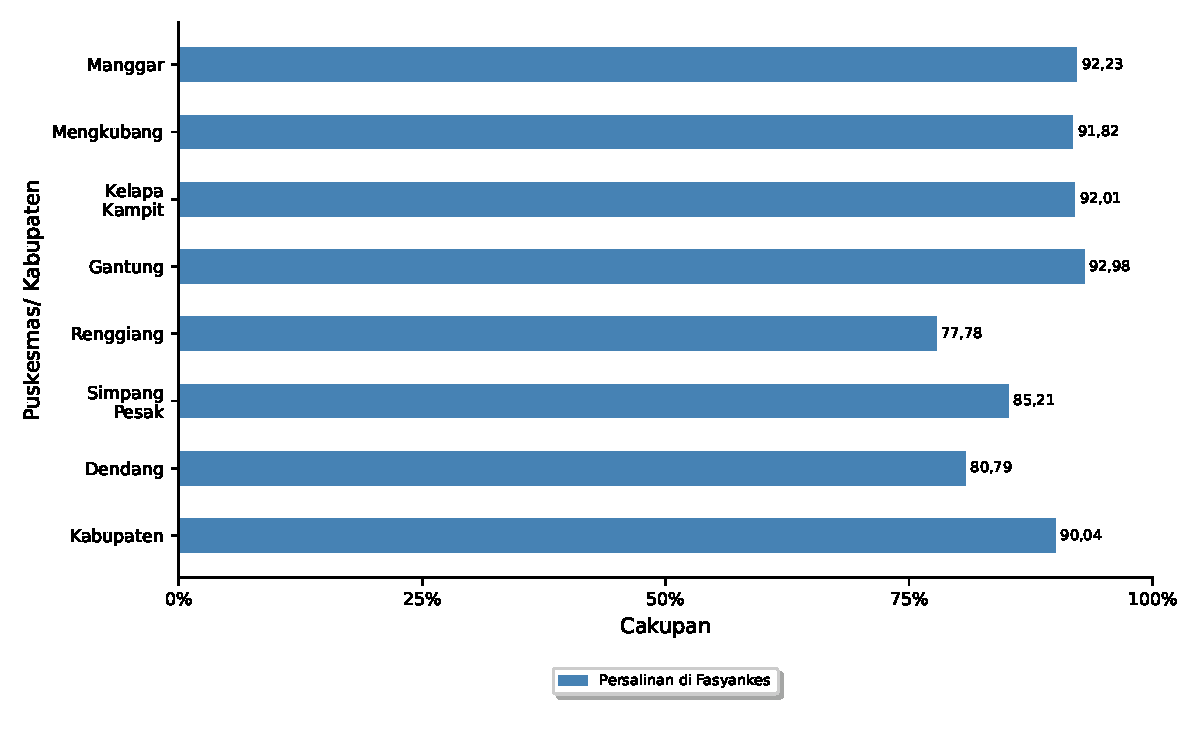
\includegraphics[width=0.9\textwidth]{bab_05/bab_05_05b_salinFasyankes.pdf}
    \caption{Cakupan Persalinan di Fasyankes di Kab. Belitung Timur Tahun \tP per Puskesmas}
    \label{fig:Cakupan-Persalinan-Fasyankes}
\end{figure}

\subsection{Pelayanan Kesehatan Nifas}
Masa nifas dimulai dari enam jam sampai dengan 42 hari pasca persalinan.
Pelayanan kesehatan nifas adalah pelayanan kepada ibu nifas sesuai standar sedikitnya 3 kali, yaitu kunjungan nifas ke-1 pada 6 jam setelah persalinan s.d 3 hari; kunjungan nifas ke-2 hari ke 4 s/d hari ke 28 setelah persalinan, kunjungan nifas ke-3 hari ke 29 s/d hari ke 42 setelah persalinan.

Cakupan pelayanan nifas KF Lengkap adalah cakupan pelayanan kepada ibu pada masa 6 jam sampai dengan 42 hari pasca bersalin sesuai standar paling sedikit 4 kali dengan distribusi waktu 6 jam sampai hari ke-2 (KF1), hari ke-3 sampai hari ke-7 (KF2), hari ke 8 sampai ke-28 (KF3) dan hari ke-29 sampai ke-42 (KF4) setelah bersalin di suatu wilayah kerja pada kurun waktu tertentu.

Cakupan pelayanan kesehatan nifas di Kabupaten Belitung Timur pada tahun \tP sebesar 89,28\% (\autoref{fig:Cakupan-Yankes-Nifas}).%, menurun dari cakupan tahun 2020 sebesar 97,43\%.

\begin{figure}[H]
    \centering{}
    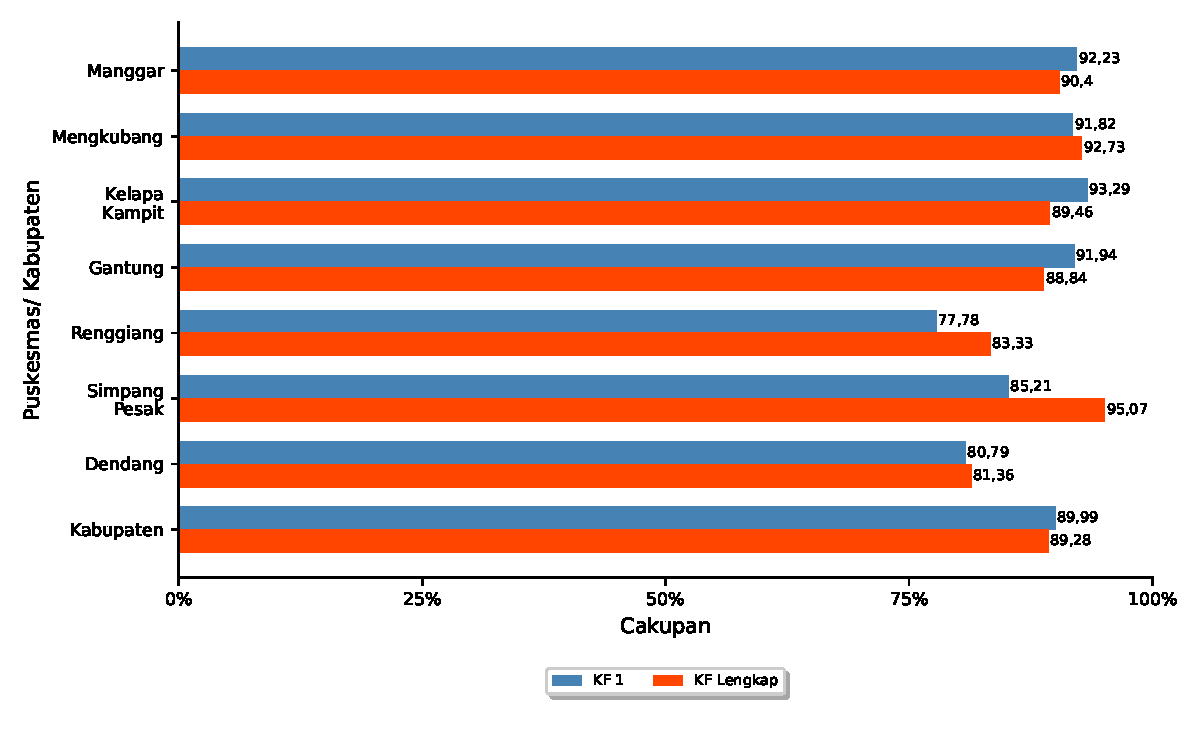
\includegraphics[width=0.9\textwidth]{bab_05/bab_05_05c_layanNifas}
    \caption{Cakupan Pelayanan Kesehatan Nifas di Kab. Belitung Timur Tahun \tP per Puskesmas}
    \label{fig:Cakupan-Yankes-Nifas}
\end{figure}

Cakupan ibu nifas mendapat vitamin A adalah cakupan ibu yang baru melahirkan atau nifas yang mendapatkan kapsul vitamin A 200.000 SI sehingga bayinya akan memperoleh vitamin A melalui ASI di satu wilayah kerja pada kurun waktu tertentu.
Cakupan ibu nifas mendapat vitamin A di Kabupaten Belitung Timur pada tahun \tP sebesar 89,57\% (\autoref{fig:Cakupan-Nifas-VitA}).

\begin{figure}[H]
    \centering{}
    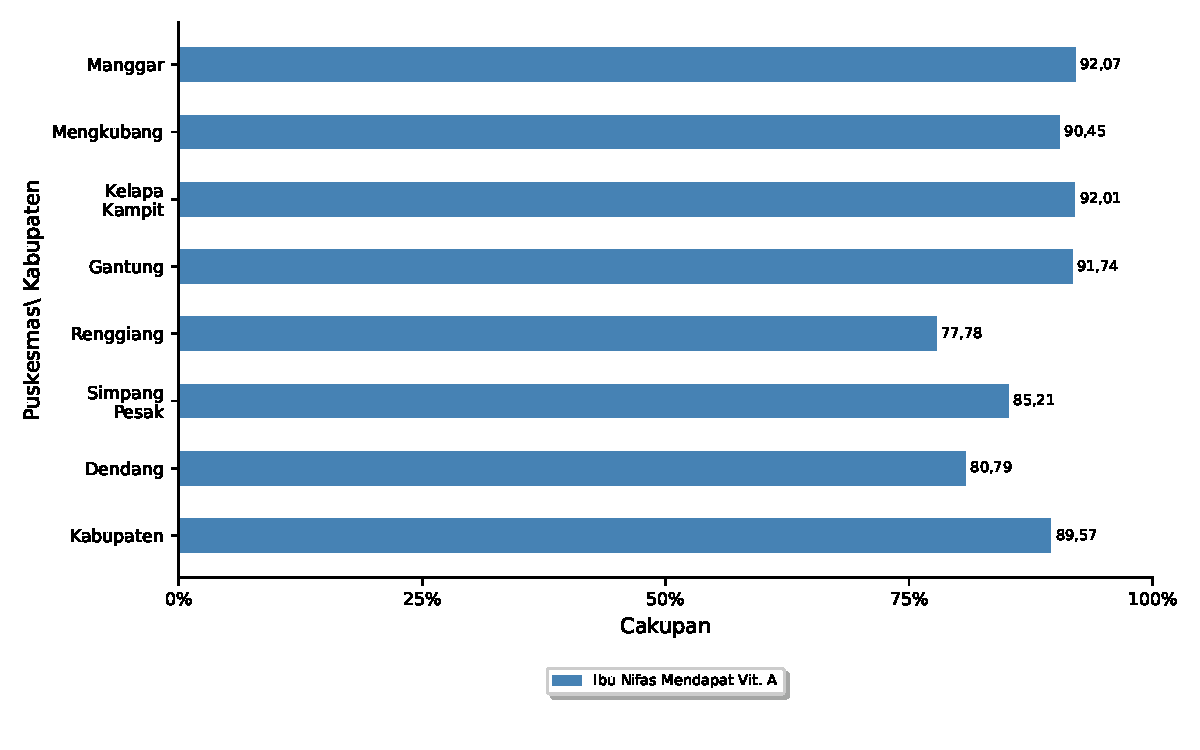
\includegraphics[width=0.9\textwidth]{bab_05/bab_05_05d_nifasVitA}
    \caption{Cakupan Ibu Nifas Mendapat Vitamin A di Kab. Belitung Timur Tahun \tP per Puskesmas}
    \label{fig:Cakupan-Nifas-VitA}
\end{figure}

\subsection{Penanganan Komplikasi Kebidanan}
Komplikasi kebidanan adalah kesakitan pada ibu hamil, ibu bersalin, ibu nifas yang dapat mengancam jiwa ibu dan/atau bayi. Sebagai salah satu faktor penyebab kematian ibu dan bayi, perlu dilakukan penanganan komplikasi kebidanan sebagai upaya menekan angka kematian ibu dan bayi.

Cakupan penanganan komplikasi kebidanan di Kabupaten Belitung Timur pada tahun \tP adalah sebesar 112,21\%,
%menurun dari cakupan tahun 2020 sebesar 133,97\% (\autoref{fig:Cakupan-Komplikasi-Kebidanan}).

\begin{figure}[H]
    \centering
    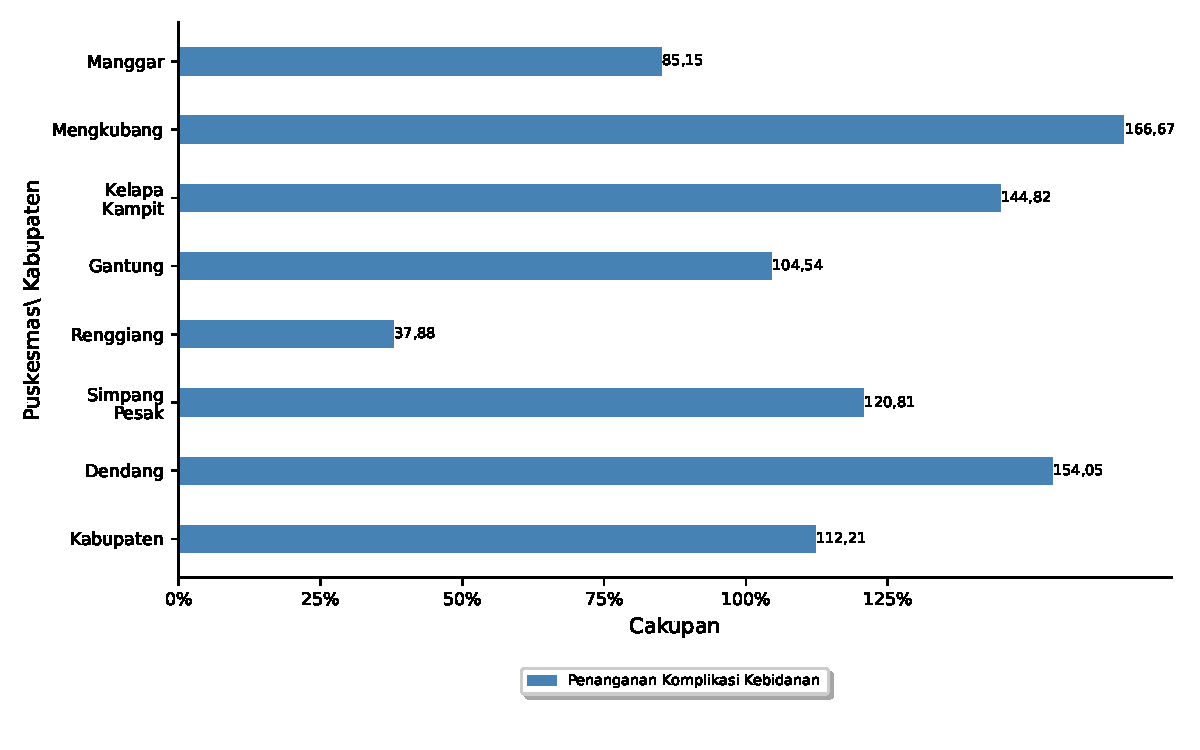
\includegraphics[width=0.9\textwidth]{bab_05/bab_05_05e_komplikasiKebidanan}
    \caption{Cakupan Penanganan Komplikasi Kebidanan di Kab. Belitung Timur Tahun \tP per Puskesmas}
    \label{fig:Cakupan-Komplikasi-Kebidanan}
\end{figure}


\subsection{Cakupan Peserta Keluarga Berencana}
Keluarga Berencana (KB) adalah upaya mengatur kelahiran anak, jarak dan usia ideal melahirkan, mengatur kehamilan, melalui promosi, perlindungan, dan bantuan sesuai dengan hak reproduksi untuk mewujudkan keluarga yang berkualitas. Program KB bertujuan untuk:
\begin{itemize}
 \item mengatur kehamilan yang diinginkan;
 \item menjaga kesehatan dan menurunkan angka kematian ibu, bayi dan anak;
 \item meningkatkan akses dan kualitas informasi, pendidikan, konseling, dan pelayanan keluarga berencana dan kesehatan reproduksi;
 \item meningkatkan partisipasi dan kesertaan pria dalam praktek keluarga berencana; dan
 \item mempromosikan penyusuan bayi sebagai upaya untuk menjarangkan jarak kehamilan.
\end{itemize}
Diharapkan dengan program KB akan dapat meningkatkan kualitas keluarga agar dapat timbul rasa aman, tenteram, dan harapan masa depan yang lebih baik dalam mewujudkan kesejahteraan lahir dan kebahagiaan batin.

\subsubsection{Cakupan peserta KB Aktif}
Peserta KB aktif adalah peserta KB baru dan lama yang masih aktif memakai kontrasepsi terus-menerus untuk menunda, menjarangkan kehamilan atau yang mengakhiri kesuburan. Cakupan peserta KB aktif di Kabupaten Belitung Timur pada tahun \tP adalah sebesar 79,03\% (\autoref{fig:Cakupan-KB-aktif-a} \& ~\autoref{fig:Cakupan-KB-aktif-b}). Metode KB yang paling banyak dipilih oleh peserta KB aktif adalah KB Suntik sebanyak 60,77 \% (\autoref{fig:Cakupan-KB-aktif-c}).

\begin{figure}[H]
    \centering
    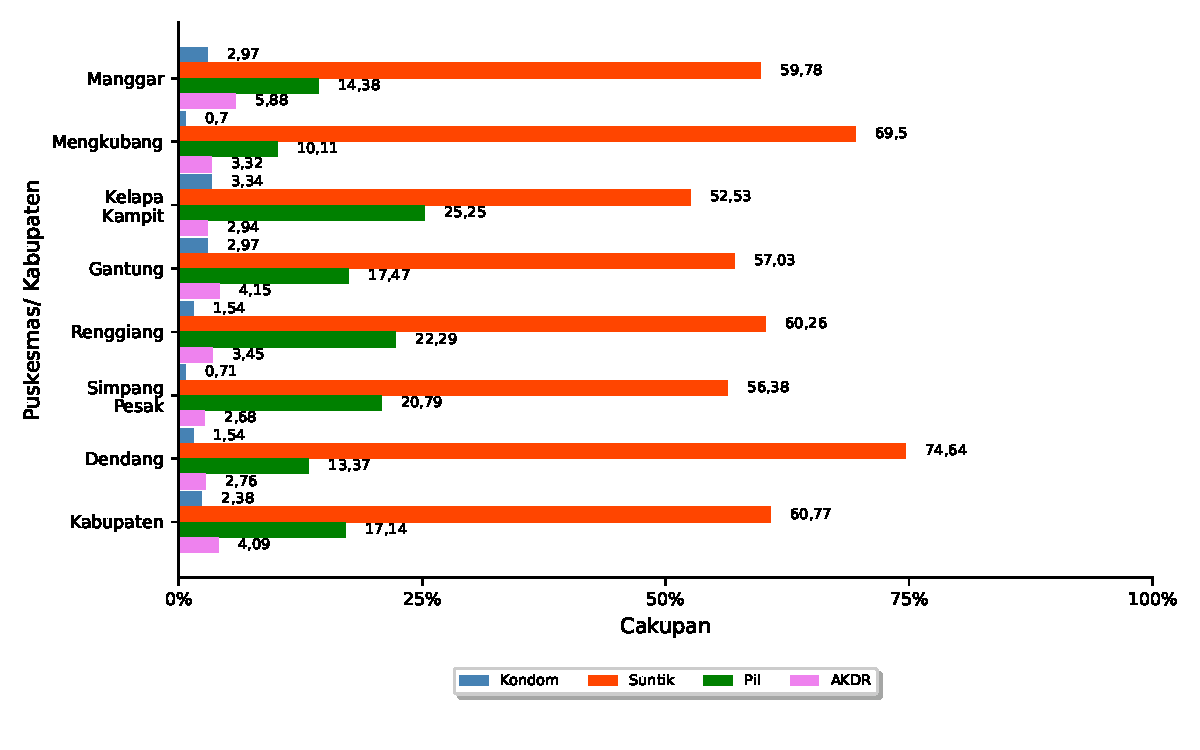
\includegraphics[width=0.9\textwidth]{bab_05/bab_05_06_KBaktif_a}
    \caption{Cakupan Peserta KB Aktif di Kab. Belitung Timur Tahun \tP per Puskesmas}
    \label{fig:Cakupan-KB-aktif-a}
\end{figure}

\begin{figure}[H]
    \centering
    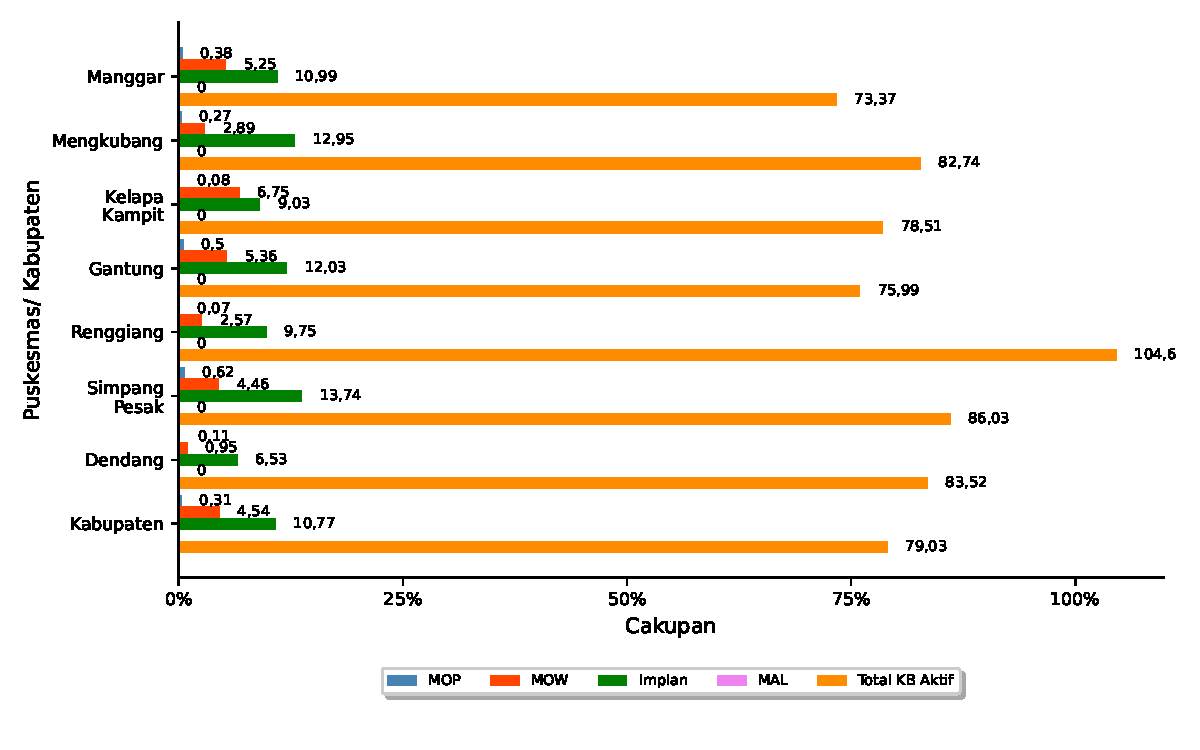
\includegraphics[width=0.9\textwidth]{bab_05/bab_05_06_KBaktif_b}
    \caption{Cakupan Peserta KB Aktif di Kab. Belitung Timur Tahun \tP per Puskesmas (lanj.)}
    \label{fig:Cakupan-KB-aktif-b}
\end{figure}

\begin{figure}[H]
    \centering
    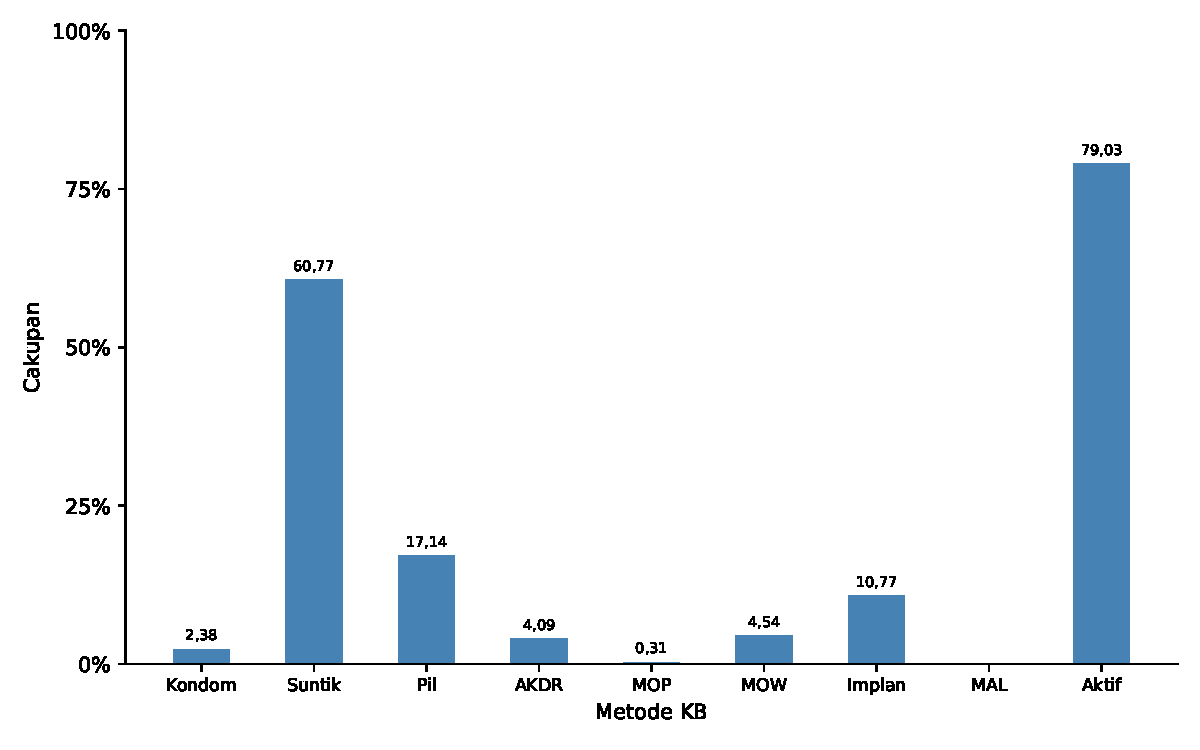
\includegraphics[width=0.9\textwidth]{bab_05/bab_05_06_KBaktif_c}
    \caption{Cakupan Metode Yang Digunakan Peserta KB Aktif di Kab. Belitung Timur Tahun \tP}
    \label{fig:Cakupan-KB-aktif-c}
\end{figure}

\subsubsection{Pasangan Usia Subur dengan status 4T dan ALKI}
Pasangan Usia Subur(PUS) dengan status 4 Terlalu (4T) adalah PUS dimana istrinya memenuhi minimal salah satu kriteria 4 Terlalu (4T), yaitu :
\begin{enumerate}
	\item berusia kurang dari 20 tahun;
	\item berusia lebih dari 35 tahun;
	\item telah memiliki anak hidup lebih dari 3 orang;atau
	\item jarak kelahiran antara satu anak dengan lainnya kurang dari 2 tahun
\end{enumerate}

Cakupan PUS dengan status 4T yang menjadi peserta KB aktif di Kabupaten Belitung Timur pada tahun \tP  adalah sebesar 14,16\% (\autoref{fig:Cakupan-4T-ALKI-menjadi-KB-Aktif}).

Pasangan Usia Subur(PUS) dengan ALKI adalah PUS yang istrinya mengalami salah satu dari gejala: Anemia, Lingkar Lengan Atas < 23,5, penyakit kronis, atau Infeksi Menular Seksual (IMS).
Penyakit kronis yang dimaksud terdiri dari Diabetes Melitus, Hipertensi, jantung, ginjal, auto imun, Hepatitis B, Thyroid, TORCH, hiperkoagulasi, stroke, Thalasemia, Hemofilia, kanker, masalah kesehatan jiwa, HIV, TBC, dan Malaria.

Cakupan PUS dengan ALKI yang menjadi peserta KB aktif di Kabupaten Belitung Timur pada tahun \tP  adalah sebesar 3,96\% (\autoref{fig:Cakupan-4T-ALKI-menjadi-KB-Aktif}).

\begin{figure}[H]
	\centering
	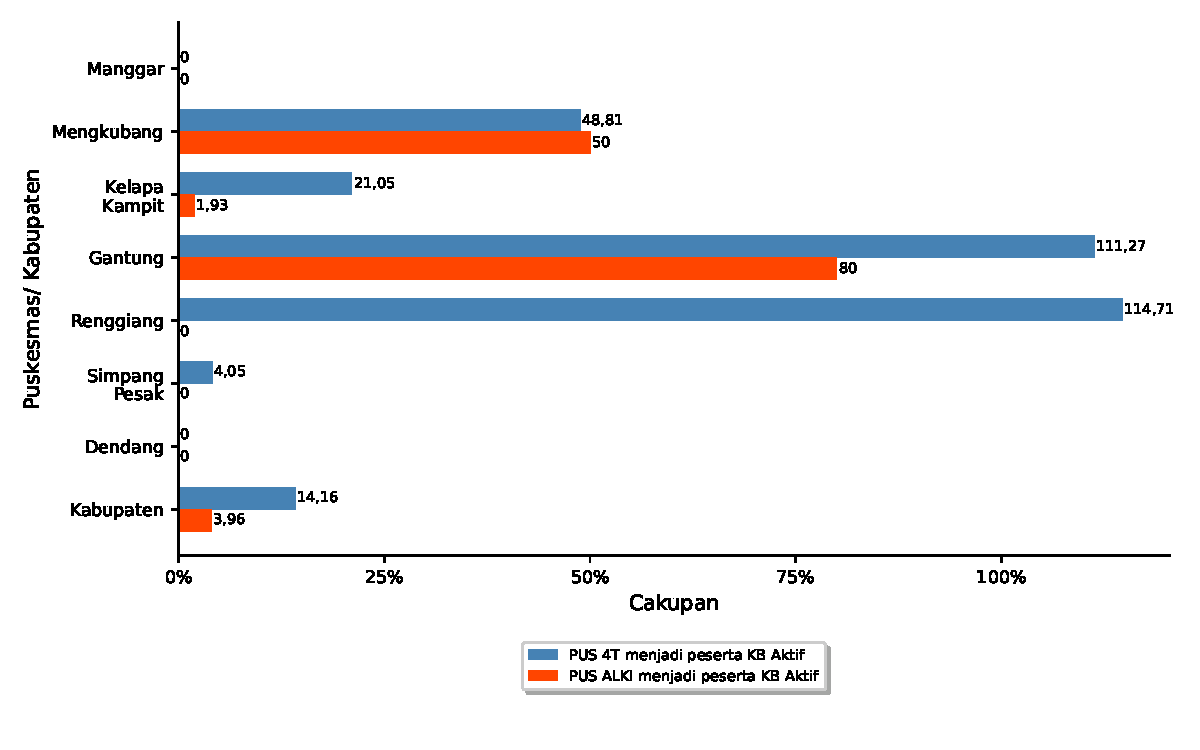
\includegraphics[width=0.9\textwidth]{bab_05/bab_05_06a_KB4TALKI}
	\caption{Cakupan PUS Dengan Status 4T dan ALKI Menjadi Peserta KB Aktif di Kab. Belitung Timur Tahun \tP}
	\label{fig:Cakupan-4T-ALKI-menjadi-KB-Aktif}
\end{figure}

\subsubsection{Cakupan peserta KB Pasca Persalinan}
Peserta KB Pasca Persalinan adalah Pasangan Usia Subur (PUS) yang memakai kontrasepsi pada masa pasca persalinan (0-42 hari setelah melahirkan). Cakupan peserta KB pasca persalinan di Kabupaten Belitung Timur pada tahun \tP adalah sebesar 73,98\% dari jumlah ibu bersalin(\autoref{fig:Cakupan-KB-pascaSalin-a} \& ~\autoref{fig:Cakupan-KB-pascaSalin-b}). Metode KB yang paling banyak dipilih oleh PUS di masa pasca persalinan adalah KB Suntik sebanyak 46,84 \% (\autoref{fig:Cakupan-KB-pascaSalin-c}).

\begin{figure}[H]
    \centering
    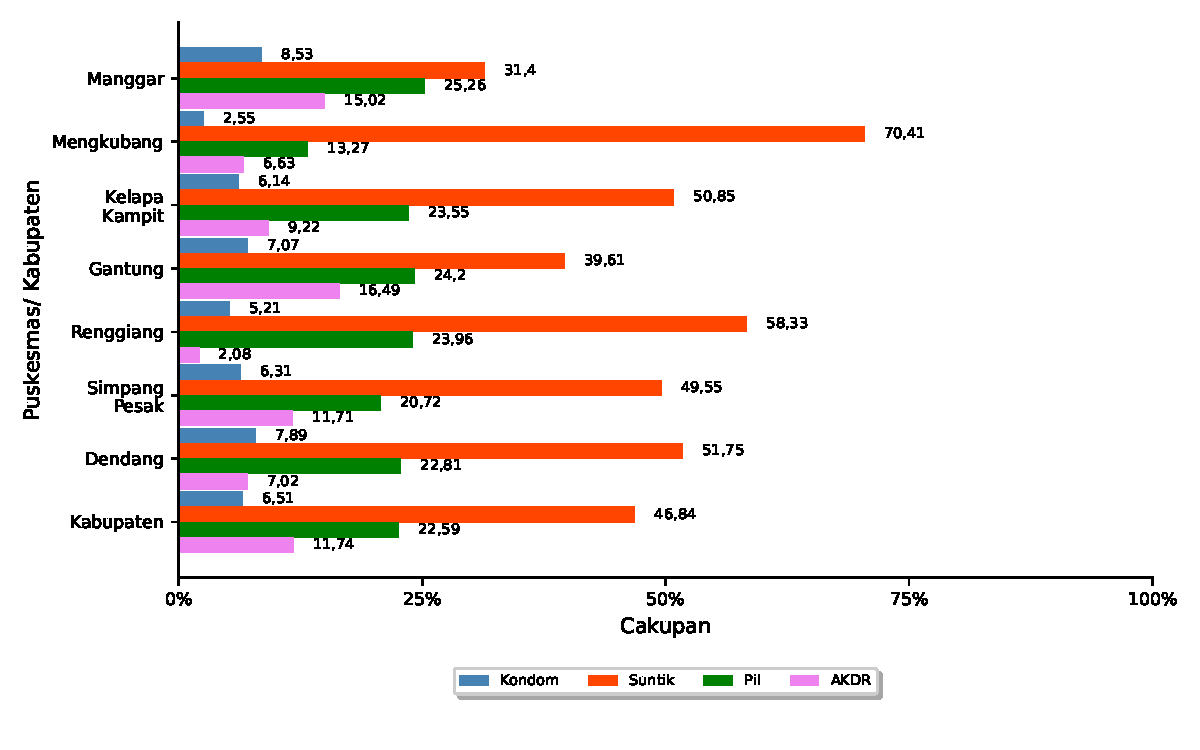
\includegraphics[width=0.85\textwidth]{bab_05/bab_05_07_KBpascaSalin_a}
    \caption{Cakupan Peserta KB Pasca Persalinan di Kab. Belitung Timur Tahun \tP per Puskesmas}
    \label{fig:Cakupan-KB-pascaSalin-a}
\end{figure}

\begin{figure}[H]
    \centering
    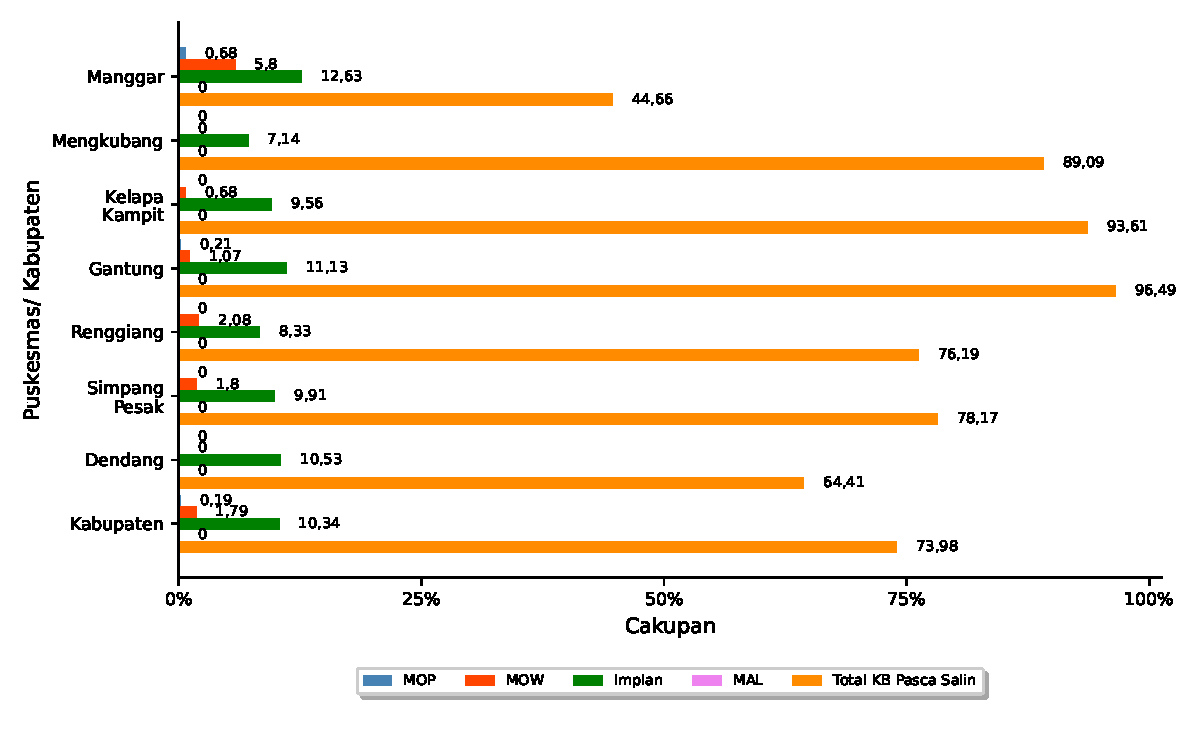
\includegraphics[width=0.85\textwidth]{bab_05/bab_05_07_KBpascaSalin_b}
    \caption{Cakupan Peserta KB Pasca Persalinan di Kab. Belitung Timur Tahun \tP per Puskesmas (lanj.)}
    \label{fig:Cakupan-KB-pascaSalin-b}
\end{figure}

\begin{figure}[H]
    \centering
    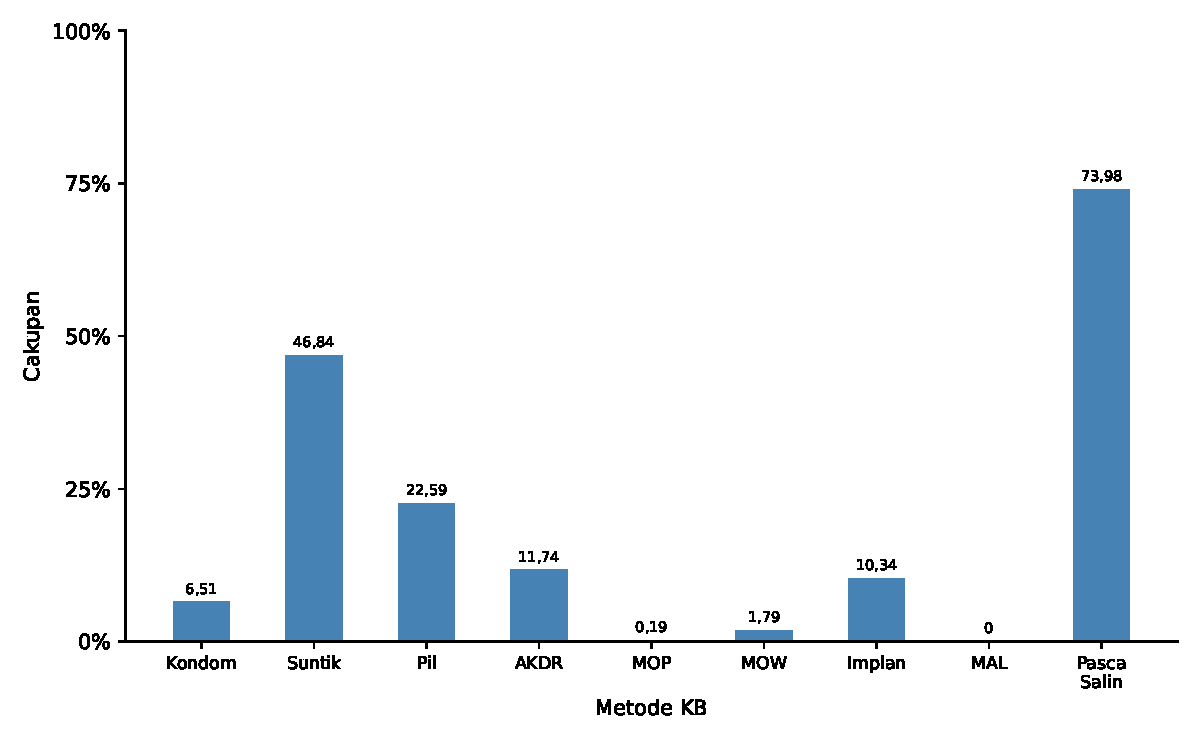
\includegraphics[width=0.9\textwidth]{bab_05/bab_05_07_KBpascaSalin_c}
    \caption{Cakupan Metode Yang Digunakan Peserta KB pasca Persalinan di Kab. Belitung Timur Tahun \tP}
    \label{fig:Cakupan-KB-pascaSalin-c}
\end{figure}

\section{KESEHATAN ANAK}
\subsection{Angka Kematian Neonatal (AKN)}
Kematian Neonatal adalah kematian yang terjadi pada bayi usia sampai dengan 28 hari tetapi bukan disebabkan oleh kecelakaan, bencana, cedera atau bunuh diri. Angka Kematian Neonatal per 1.000 kelahiran hidup adalah jumlah bayi usia sampai dengan 28 hari yang meninggal di suatu wilayah pada kurun waktu tertentu per 1.000 jumlah kelahiran hidup di wilayah dan pada kurun waktu yang sama.

Jumlah Kematian Neonatus yang terjadi di Kabupaten Belitung Timur sepanjang tahun \tP berjumlah 14 kematian (\autoref{fig:Jumlah-Kematian-Neonatal}). Angka Kematian Neonatal (AKN) pada tahun \tP sebesar 7,35 per 1.000 kelahiran hidup, mengalami penurunan dari tahun 2022 sebesar 8,39 per 1.000 kelahiran hidup (\autoref{fig:AKN-2019-2023}).

\begin{figure}[H]
    \centering{}
    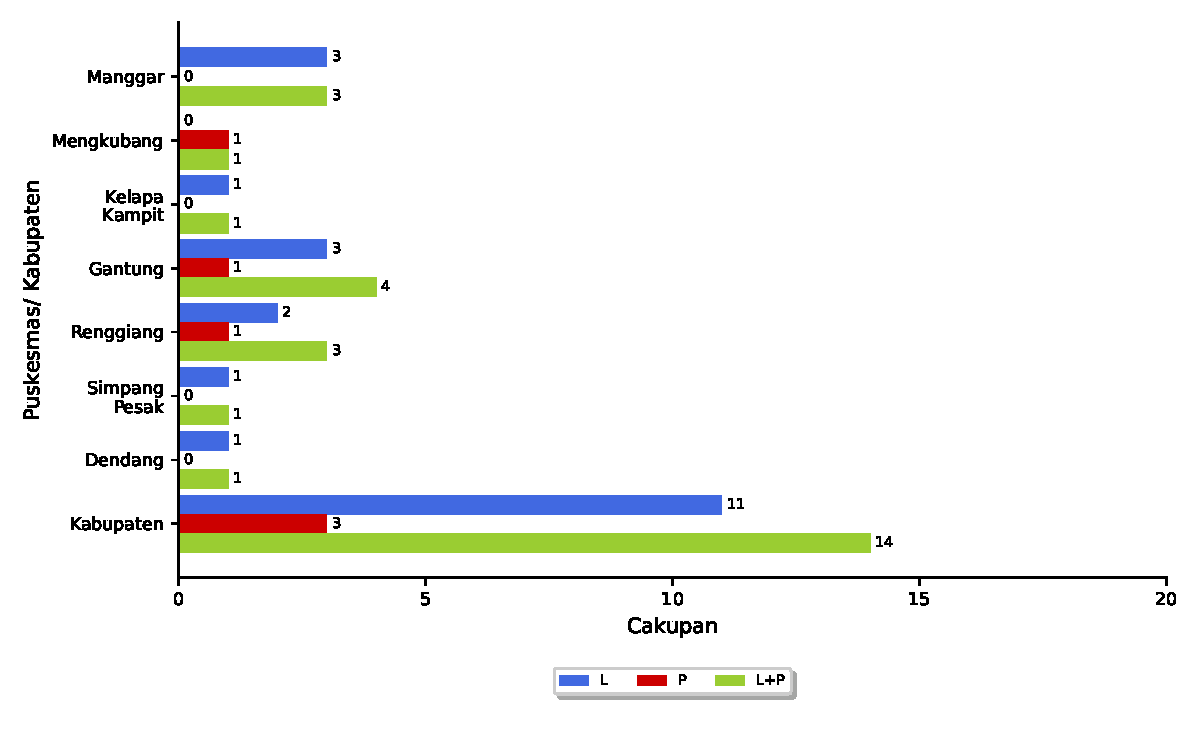
\includegraphics[width=0.85\textwidth]{bab_05/bab_05_09_kematianNeonatal}
    \caption{Jumlah Kematian Neonatal di Kab. Belitung Timur Tahun \tP per Puskesmas}
    \label{fig:Jumlah-Kematian-Neonatal}
\end{figure}

\begin{figure}[H]
    \centering{}
    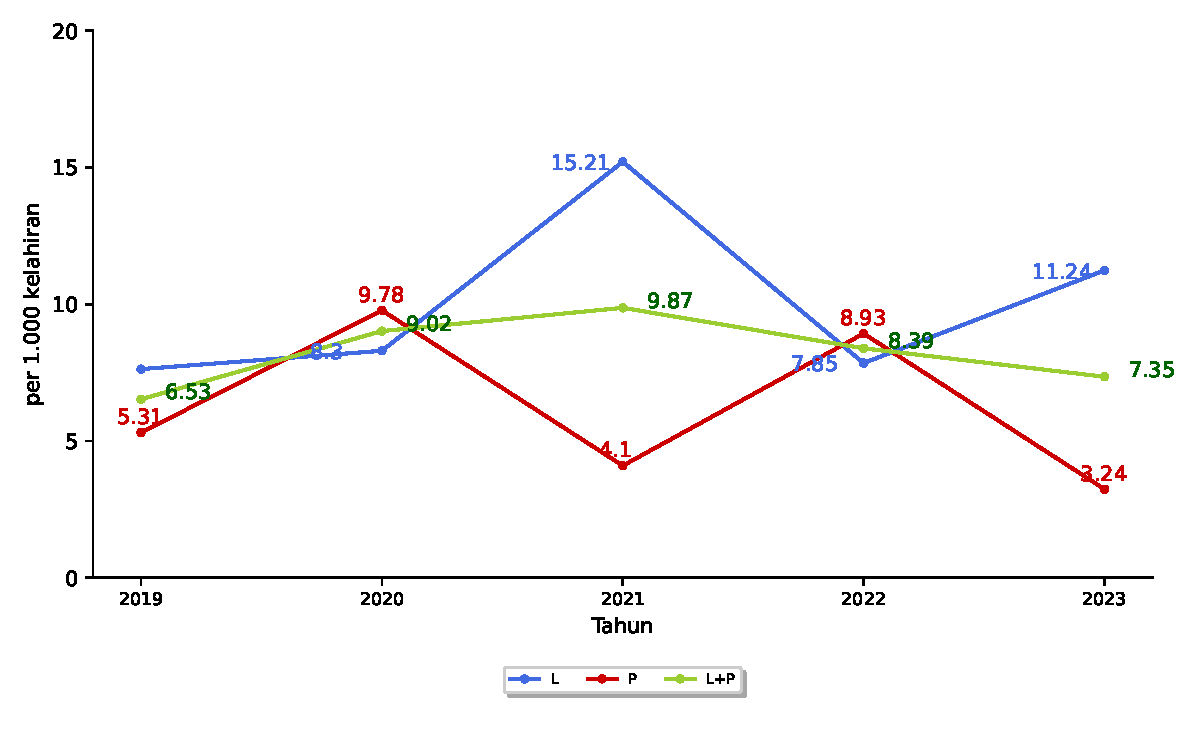
\includegraphics[width=0.85\textwidth]{bab_05/bab_05_09_plotNeonatal}
    \caption{AKN Kab. Belitung Timur Tahun 2019-2023}
    \label{fig:AKN-2019-2023}
\end{figure}


\subsection{Angka Kematian Bayi (AKB)}
Kematian Bayi adalah kematian yang terjadi pada seorang bayi yang usianya sebelum mencapai satu tahun (usia 0-11 bulan, mencakup neonatal dan postnatal) tetapi bukan disebabkan oleh kecelakaan, bencana, cedera atau bunuh diri. Angka Kematian Bayi per 1.000 kelahiran hidup adalah jumlah bayi usia sampai dengan 11 bulan yang meninggal di suatu wilayah pada kurun waktu tertentu per 1.000 jumlah kelahiran hidup di wilayah dan pada kurun waktu yang sama.

Jumlah Kematian Bayi yang terjadi di Kabupaten Belitung Timur sepanjang tahun \tP berjumlah 17 kematian (\autoref{fig:Jumlah-Kematian-Bayi}). Angka Kematian Bayi (AKB) pada tahun \tP adalah sebesar 8,92 per 1.000 kelahiran hidup, mengalami penurunan dari AKB tahun 2022 sebesar 12,30 per 1.000 kelahiran hidup (\autoref{fig:AKB-2019-2023}).

\begin{figure}[H]
    \centering{}
    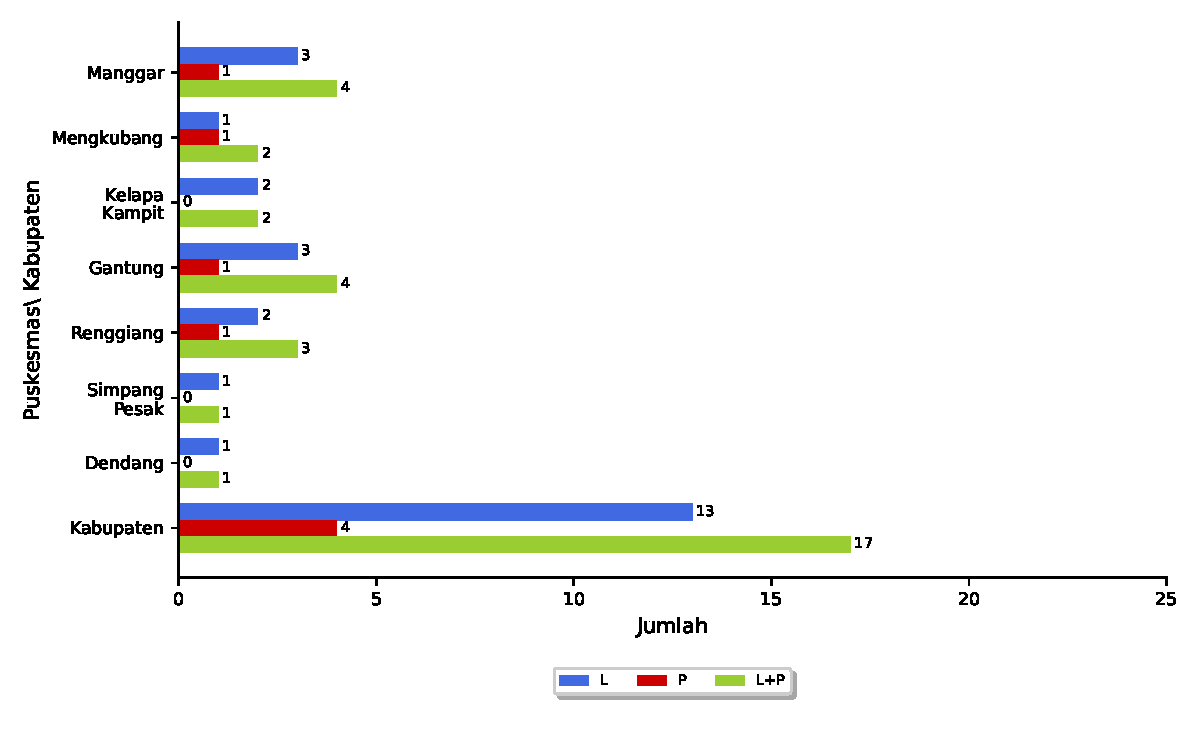
\includegraphics[width=0.85\textwidth]{bab_05/bab_05_10_kematianBayi}
    \caption{Jumlah Kematian Bayi di Kab. Belitung Timur Tahun \tP per Puskesmas}
    \label{fig:Jumlah-Kematian-Bayi}
\end{figure}

\begin{figure}[H]
    \centering{}
    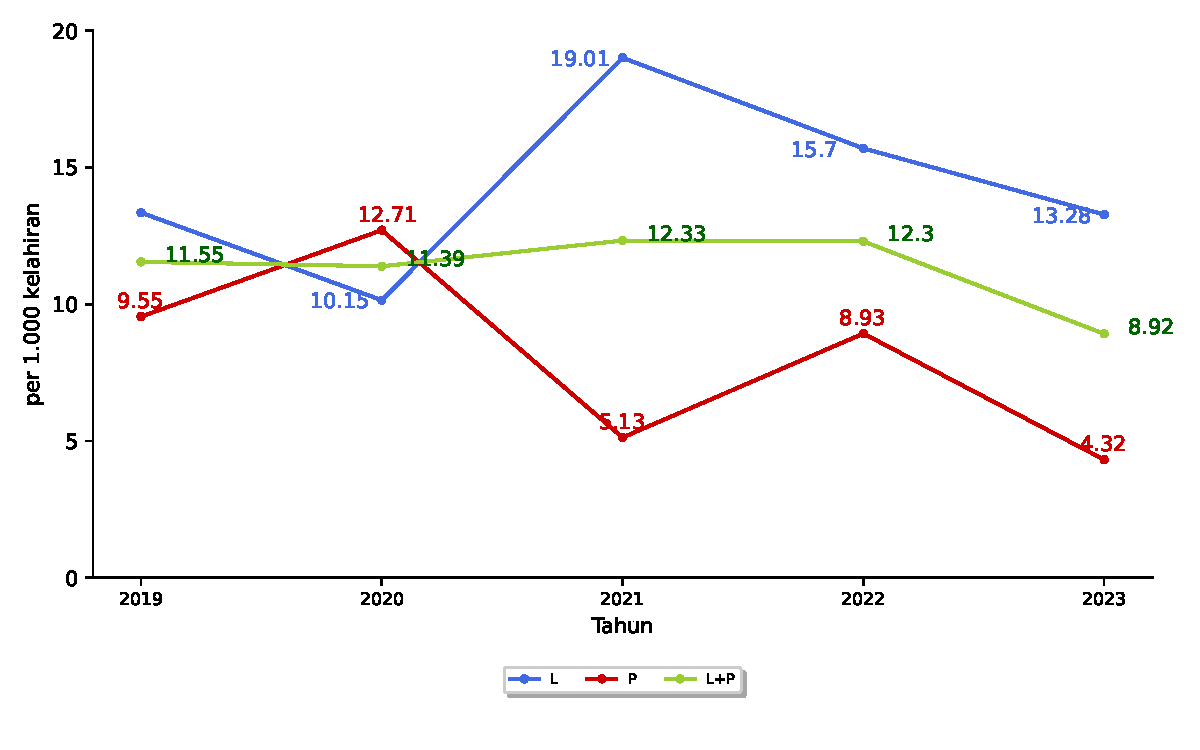
\includegraphics[width=0.85\textwidth]{bab_05/bab_05_10_plotBayi}
    \caption{AKB Kab. Belitung Timur Tahun 2019-2023}
    \label{fig:AKB-2019-2023}
\end{figure}


\subsection{Angka Kematian Balita (AKBA)}
Kematian Balita adalah kematian yang terjadi pada bayi/anak usia 0 - 59 bulan (bayi + anak balita) tetapi bukan disebabkan oleh kecelakaan, bencana, cedera atau bunuh diri. Angka Kematian Balita (AKBA) adalah jumlah balita usia 59 bulan (mencakup bayi dan anak balita) yang meninggal di suatu wilayah pada kurun waktu tertentu
per 1.000 jumlah kelahiran hidup di wilayah pada kurun waktu yang sama.

Jumlah Kematian Balita yang terjadi di Kabupaten Belitung Timur sepanjang tahun \tP berjumlah 19 kematian (\autoref{fig:Jumlah-Kematian-Balita}). Angka Kematian Balita (AKBA) pada tahun \tP sebesar 9,97 per 1.000 kelahiran hidup, mengalami penurunan dari AKBA tahun 2022 sebesar 14,54 per 1.000 kelahiran hidup (\autoref{fig:AKBA-2019-2023}).

\begin{figure}[H]
    \centering{}
    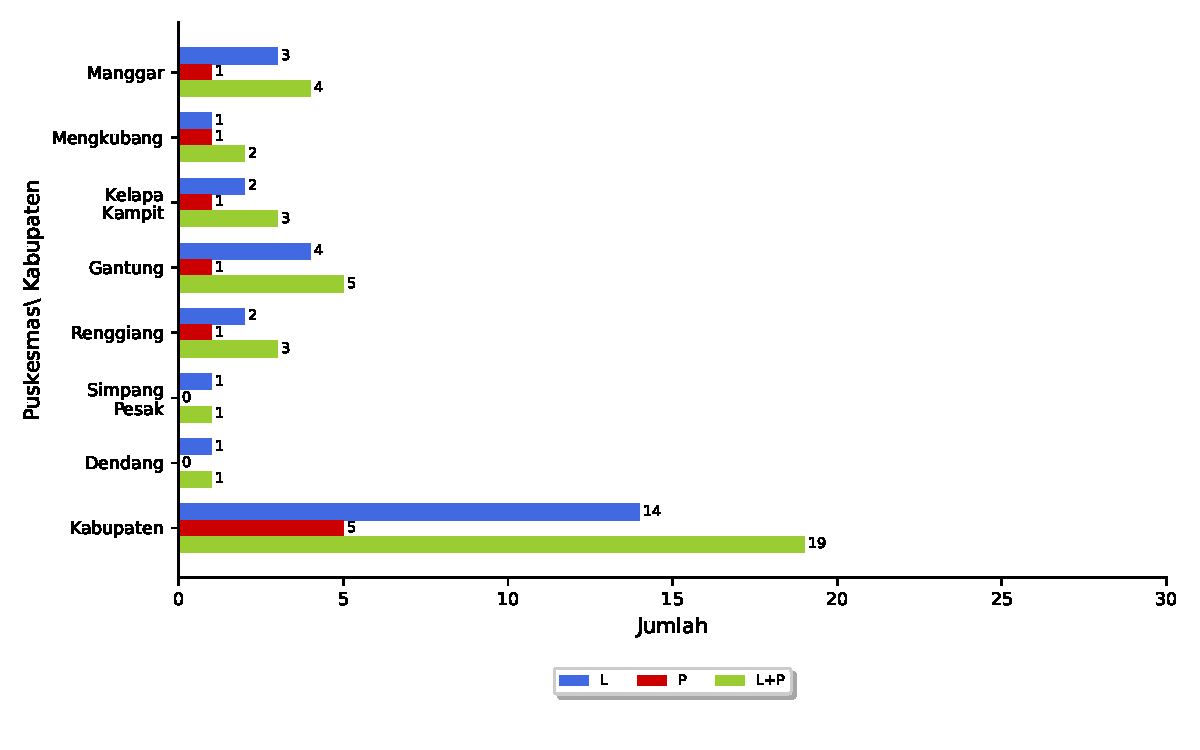
\includegraphics[width=0.85\textwidth]{bab_05/bab_05_11_kematianBalita}
    \caption{Jumlah Kematian Balita di Kabupaten Belitung Timur Tahun \tP per Puskesmas}
    \label{fig:Jumlah-Kematian-Balita}
\end{figure}

\begin{figure}[H]
    \centering{}
    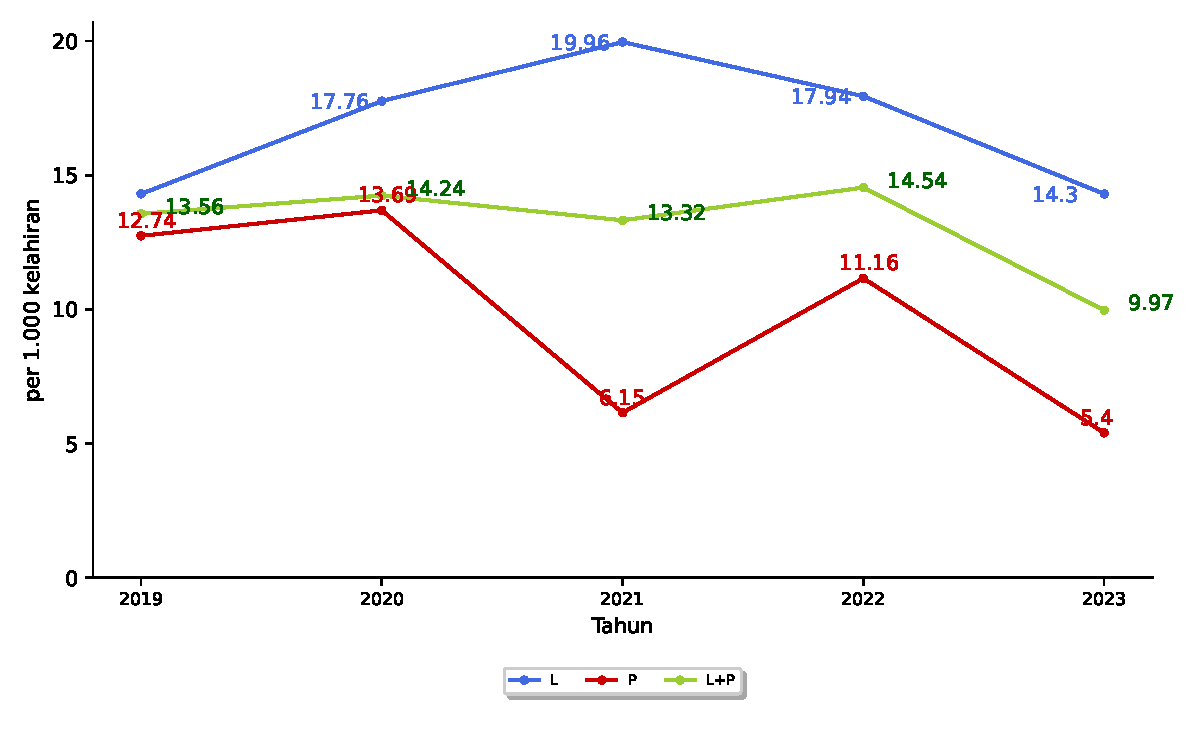
\includegraphics[width=0.8\textwidth]{bab_05/bab_05_11_plotBalita}
    \caption{AKABA Kabupaten Belitung Timur 2019-2023}
    \label{fig:AKBA-2019-2023}
\end{figure}

\begin{figure}[H]
    \centering{}
    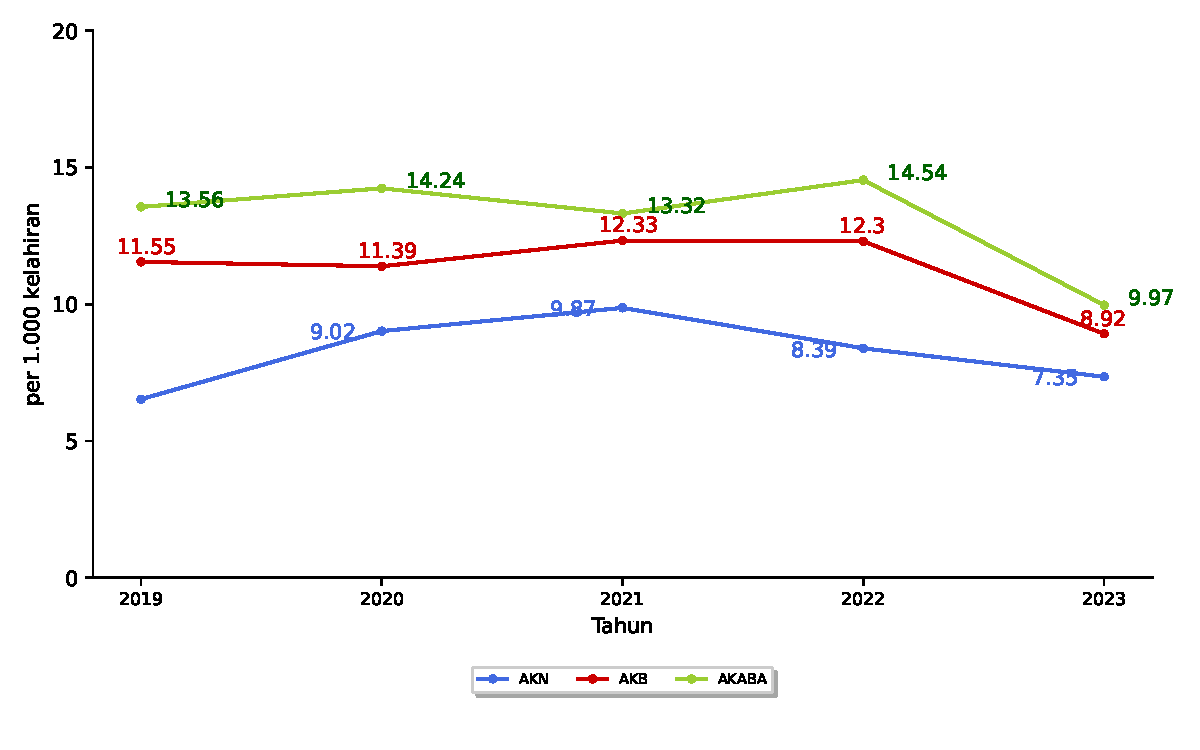
\includegraphics[width=0.8\textwidth]{bab_05/bab_05_11a_plotNeoBayiBalita}
    \caption{AKN, AKB dan AKBA Kabupaten Belitung Timur 2019-2023}
    \label{fig:AKN-AKB-AKBA-2019-2023}
\end{figure}

\subsection{Penanganan Komplikasi Neonatal}
Komplikasi neonatal adalah neonatal dengan penyakit dan kelainan yang
dapat menyebabkan kesakitan, kecacatan, dan kematian neonatus dengan
komplikasi seperti BBLR (berat badan lahir rendah < 2500 gr), asfiksia, infeksi, tetanus neonatorum, kelainan kongenital, Covid 19, dan lain-lain
seperti ikterus, hipotermia, trauma lahir, sindroma gangguan pernafasan. Penanganan neonatal dengan komplikasi adalah
penanganan terhadap neonatal sakit dan atau neonatal dengan kelainan
atau komplikasi/kegawatdaruratan yang mendapat pelayanan sesuai standar
oleh tenaga kesehatan terlatih di seluruh sarana pelayanan kesehatan.
Pelayanan sesuai standar antara lain sesuai dengan standar MTBM, Manajemen
Asfiksia Bayi Baru Lahir, Manajemen Bayi Berat Lahir Rendah, pedoman
pelayanan neonatal essensial di tingkat pelayanan kesehatan dasar,
PONED, PONEK atau standar operasional pelayanan lainnya.

Cakupan penanganan komplikasi neonatal di Kabupaten Belitung Timur
pada tahun \tP adalah sebesar 56,22\%.
%menurun dari cakupan tahun2020 sebesar 78,26\% (\autoref{fig:Pelayanan-Komplikasi-Neonatal}).

\begin{figure}[H]
    \centering
    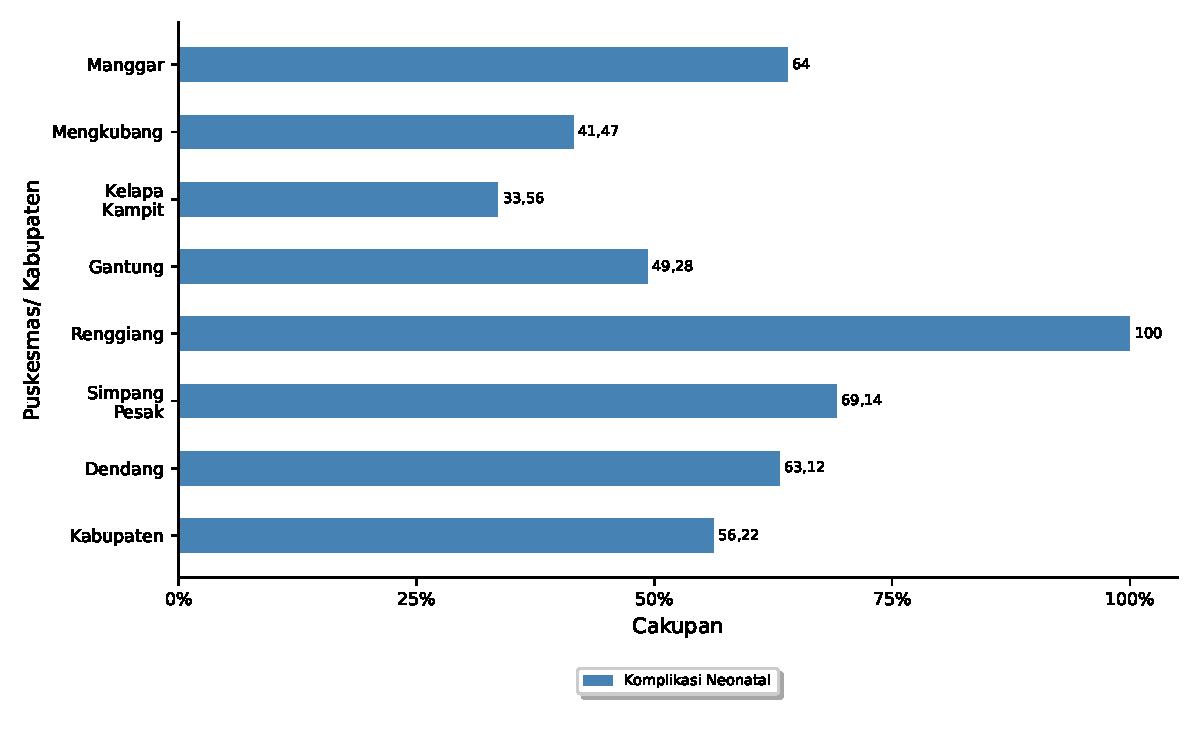
\includegraphics[width=0.85\textwidth]{bab_05/bab_05_12_komplikasiNeonatal}
    \caption{Cakupan Penanganan Komplikasi Neonatal di Kab. Belitung Timur Tahun \tP per Puskesmas}
    \label{fig:Pelayanan-Komplikasi-Neonatal}
\end{figure}


\subsection{Berat Badan Bayi Lahir Rendah (BBLR) dan Bayi Prematur}
Berat Badan Bayi Lahir Rendah adalah berat badan bayi kurang dari
2500 gram. BBLR dibedakan menjadi 2 (dua) kategori yaitu BBLR karena
prematur (kurang dari 37 minggu) dan BBLR karena \emph{Intrauterine Growth Restriction}(IUGR), yaitu bayi yang lahir cukup bulan tetapi berat badannya kurang.

Pada tahun \tP, tercatat bahwa Berat Badan Bayi Lahir Rendah adalah berjumlah
146 kasus atau 7,66\% dari jumlah kelahiran hidup (\autoref{fig:Distribusi-BBLR}).
%menurun dari cakupan tahun 2021 sebesar 5,53\%.

\begin{figure}[H]
  \centering
  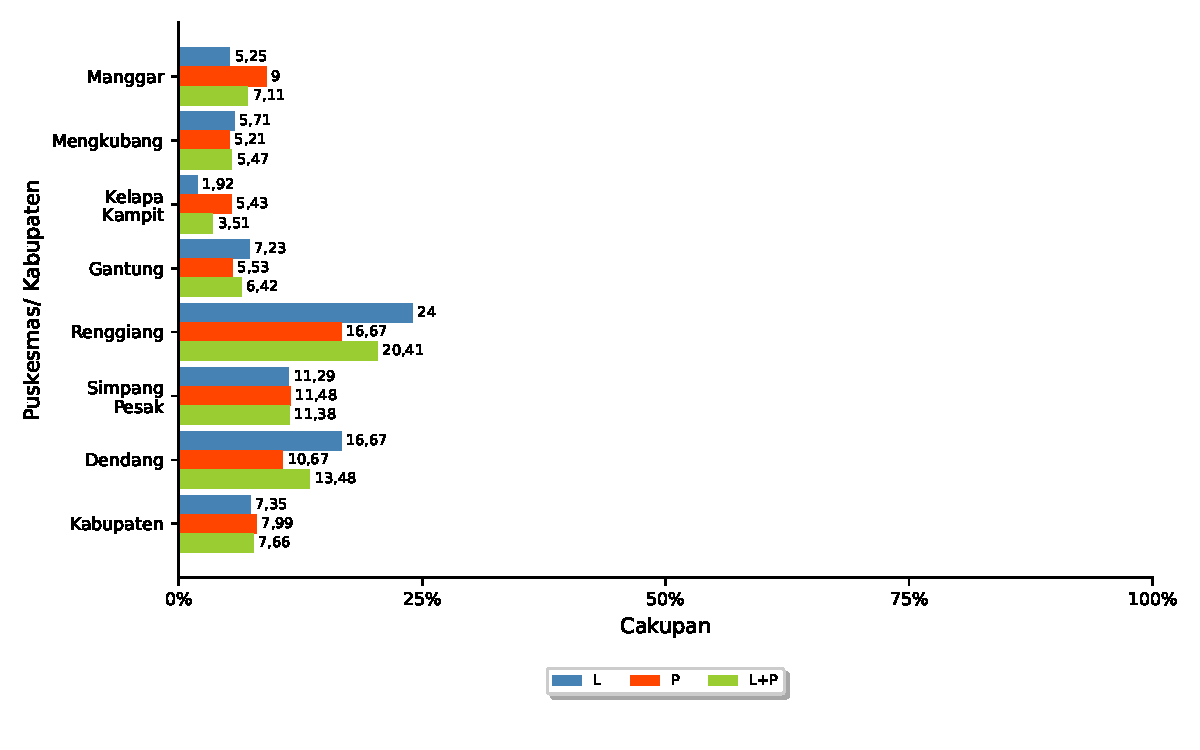
\includegraphics[width=0.85\textwidth]{bab_05/bab_05_13_BBLR}
  \caption{Sebaran BBLR di Kab. Belitung Timur Tahun \tP per Puskesmas}
  \label{fig:Distribusi-BBLR}
\end{figure}

Pada tahun \tP, tercatat bahwa Bayi Lahir Prematur adalah berjumlah
137 kasus atau 6,80\% dari jumlah kelahiran hidup (\autoref{fig:Distribusi-Prematur}).

\begin{figure}[H]
	\centering
	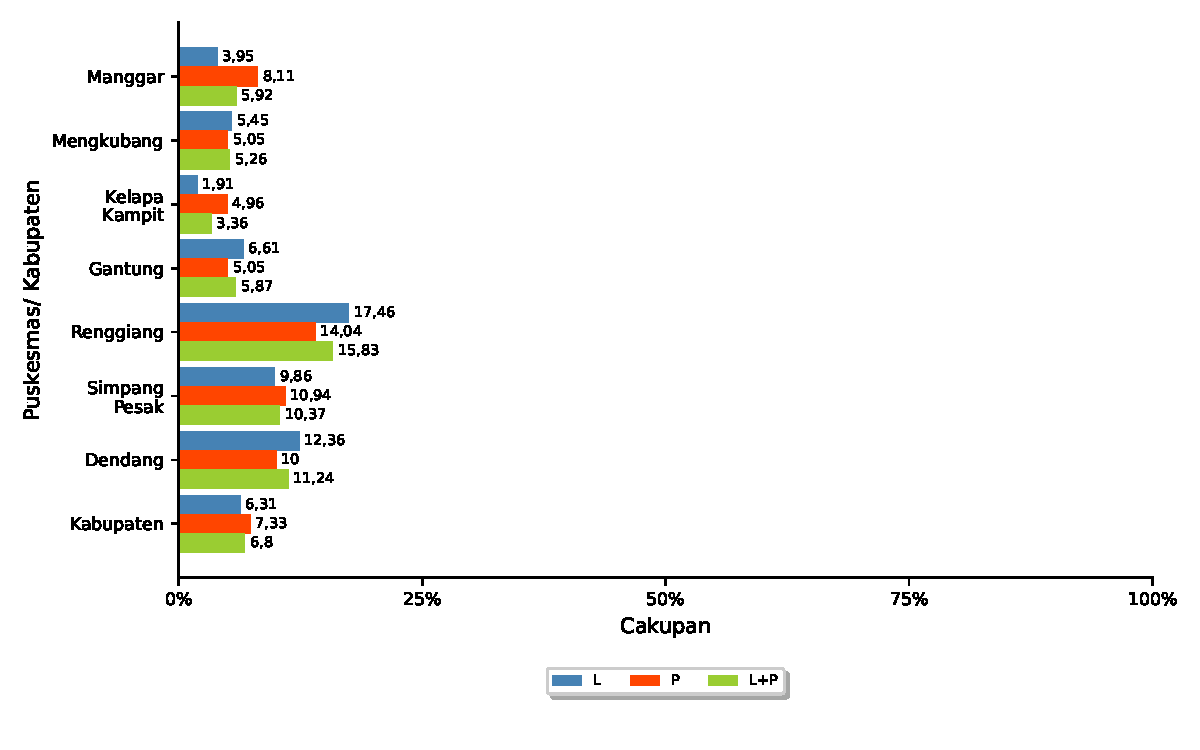
\includegraphics[width=0.85\textwidth]{bab_05/bab_05_13a_Prematur}
	\caption{Sebaran Bayi Lahir Prematur di Kab. Belitung Timur Tahun \tP per Puskesmas}
	\label{fig:Distribusi-Prematur}
\end{figure}

\subsection{Pelayanan Kesehatan Neonatal}
Neonatus adalah bayi baru lahir yang berusia sampai dengan 28 hari.
Pada masa tersebut terjadi perubahan yang sangat besar dari kehidupan
di dalam rahim dan terjadi pematangan organ hampir pada semua sistem.
Beberapa upaya kesehatan dilakukan untuk mengendalikan risiko pada
kelompok ini di antaranya dengan mengupayakan agar persalinan dapat
dilakukan oleh tenaga kesehatan di fasilitas kesehatan serta menjamin
tersedianya pelayanan kesehatan sesuai standar pada kunjungan bayi
baru lahir.

Indikator yang menggambarkan upaya kesehatan yang dilakukan untuk
mengurangi risiko kematian pada periode neonatal yaitu cakupan KN1
dan KN Lengkap. KN1 adalah pelayanan kunjungan neonatal pertama pada
6-48 jam setelah lahir sesuai standar di satu wilayah kerja. KN Lengkap
yaitu pelayanan kunjungan neonatal lengkap, minimal 3 kali yaitu 1
kali pada usia 6 - 48 jam, 1 kali pada 3 - 7 hari, dan 1 kali pada
8 - 28 hari sesuai standar.

%Cakupan penanganan KN1 di Kabupaten Belitung Timur
%pada tahun \tP sebesar 100,00\%, meningkat
%dari cakupan tahun 2019 sebesar 99,90\%. Sedangkan cakupan penanganan KN Lengkap di Kabupaten Belitung Timur
%pada tahun \tP 98,67\%, menurun
%dari cakupan tahun 2019 sebesar 99,60\% (\autoref{fig:Cakupan-KN1-KNlengkap} dan \autoref{fig:KN1-KNlengkap-2016-2020}).

Cakupan penanganan KN1 di Kabupaten Belitung Timur pada tahun \tP sebesar 94,25\%.
Sedangkan cakupan penanganan KN Lengkap di Kabupaten Belitung Timur pada tahun \tP sebesar 94,30\% (\autoref{fig:Cakupan-KN1-KNlengkap}

% dan \autoref{fig:KN1-KNlengkap-2016-2020}).

\begin{figure}[H]
    \centering
    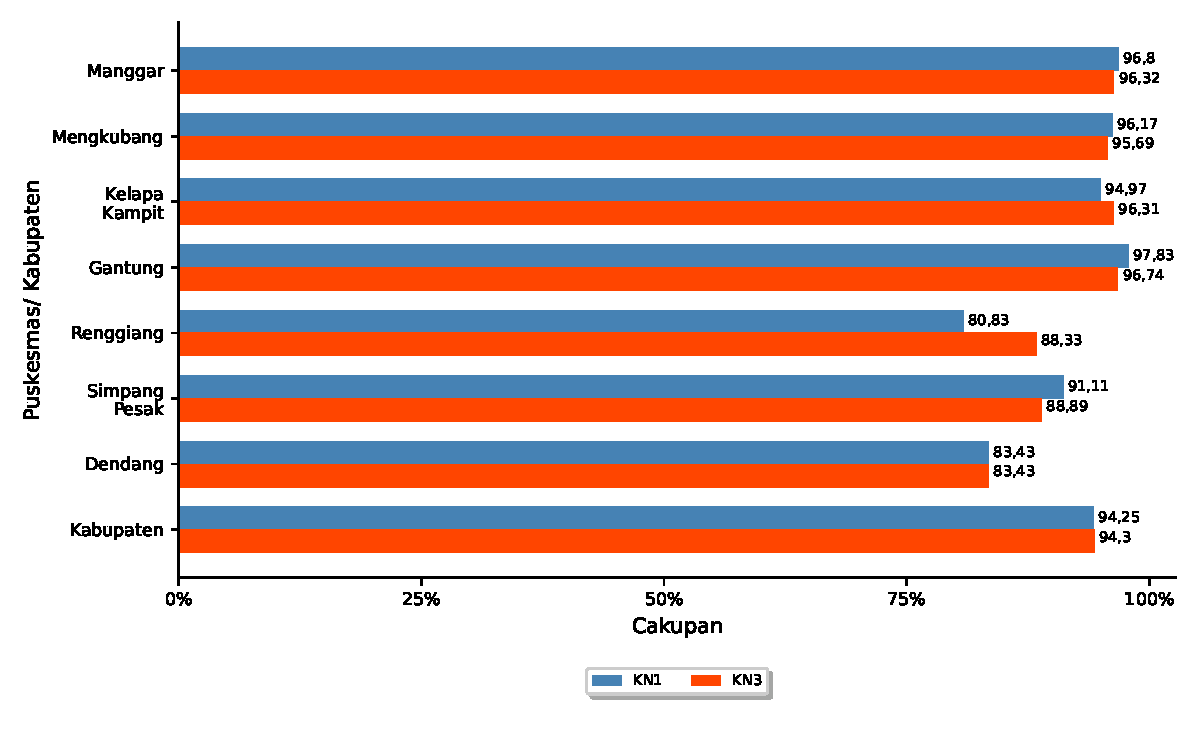
\includegraphics[width=0.9\textwidth]{bab_05/bab_05_14_KN1KN3}
    \caption{Cakupan KN1 dan KN Lengkap di Kabupaten Belitung Timur tahun \tP per Puskesmas}
    \label{fig:Cakupan-KN1-KNlengkap}
\end{figure}

%\begin{figure}[H]
%    \centering
%%%    \includegraphics[width=0.9\textwidth]{bab_05/bab_05_14a_plotKN1KN3}
%    \caption{Cakupan KN1 dan KN Lengkap di Kab. Belitung Timur Tahun 2017-2021}
%    \label{fig:KN1-KNlengkap-2016-2020}
%\end{figure}

Hipotiroid Kongenital adalah gangguan defisiensi hormon tiroid yang timbul pada bayi baru lahir yang dapat menimbulkan gangguan tumbuh kembang pada bayi.
Skrining Hipotiroid Kongenital (SHK) dilakukan dengan mengambil spesimen darah pada tumit bayi baru lahir berusia minimal 48 sampai 72 jam dan maksimal 2 minggu.

Cakupan SHK di Kabupaten Belitung Timur pada tahun \tP adalah sebesar 72,42\%.

\begin{figure}[H]
	\centering
	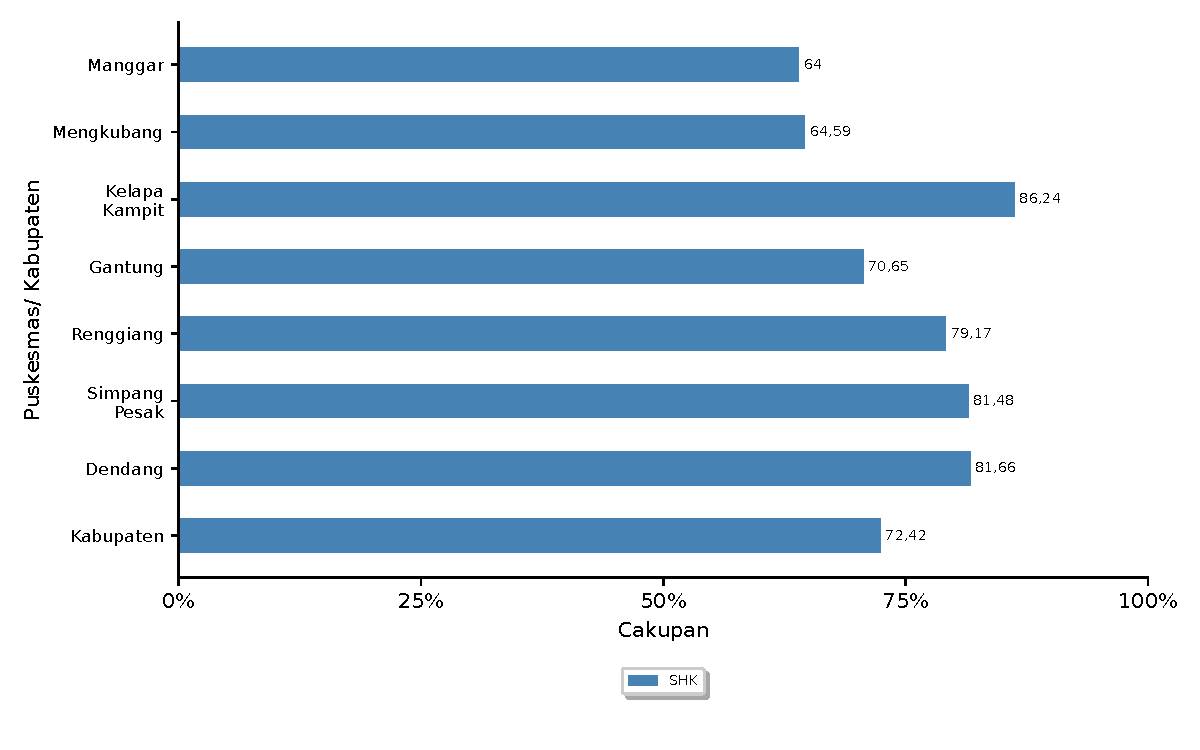
\includegraphics[width=0.9\textwidth]{bab_05/bab_05_14c_SHK}
	\caption{Cakupan SHK di Kabupaten Belitung Timur tahun \tP per Puskesmas}
	\label{fig:Cakupan-SHK}
\end{figure}

\subsection{Bayi Mendapat ASI Eksklusif}
Air Susu Ibu (ASI) adalah cairan hasil sekresi kelenjar payudara ibu
untuk konsumsi bayi dan merupakan sumber gizi utama bayi yang belum
dapat mencerna makanan padat. ASI eksklusif berdasarkan Peraturan
Pemerintah Nomor 33 Tahun 2012 adalah ASI yang diberikan kepada bayi
sejak dilahirkan selama enam bulan, tanpa menambahkan dan/atau mengganti
dengan makanan atau minuman lain (kecuali obat, vitamin, dan mineral).

Cakupan bayi mendapat ASI eksklusif di kabupaten Belitung Timur pada
tahun \tP yaitu sebesar 46,96\% (\autoref{fig:Cakupan-Bayi-ASI-Eksklusif}).
% meningkat dari cakupan tahun 2021 sebesar 45,62\%.

\begin{figure}[H]
  \centering
  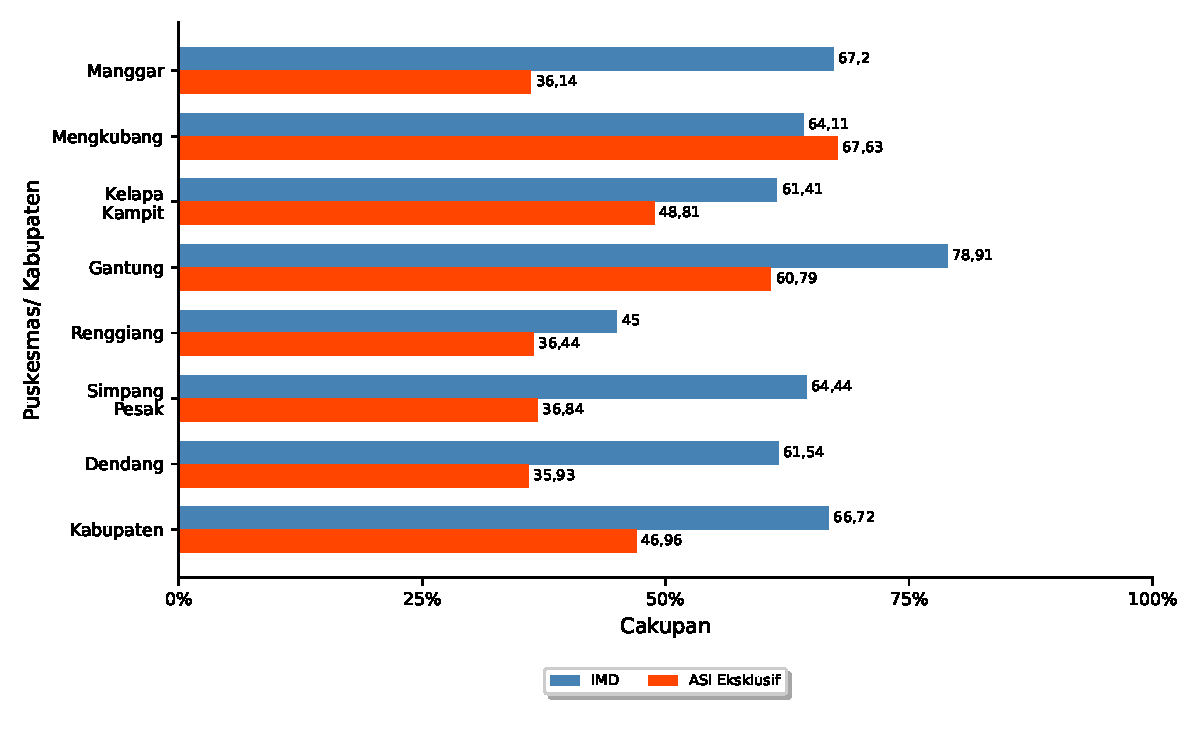
\includegraphics[width=0.9\textwidth]{bab_05/bab_05_15_ASIeksklusif}
  \caption{Cakupan Bayi Mendapat ASI Eksklusif di Kab. Belitung Timur Tahun \tP per Puskesmas}
  \label{fig:Cakupan-Bayi-ASI-Eksklusif}
\end{figure}

\subsection{Pelayanan Kesehatan Bayi}
Pelayanan kesehatan bayi adalah pelayanan kesehatan pada bayi minimal
4 kali yaitu satu kali pada umur 29 hari-2 bulan, 1 kali pada umur
3-5 bulan, 1 kali pada umur 6-8 bulan, dan 1 kali pada umur 9-11 bulan.
Pelayanan Kesehatan tersebut meliputi pemberian imunisasi dasar (BCG,
DPT/HB1-3, Polio 1-4, Campak), pemantauan pertumbuhan, Stimulasi Deteksi
Intervensi Dini Tumbuh Kembang (SDIDTK), pemberian vitamin A pada
bayi umur 6-11 bulan, penyuluhan pemberian ASI eksklusif dan Makanan
Pendamping ASI (MP ASI).

Cakupan pelayanan kesehatan bayi di Kabupaten Belitung Timur pada
tahun \tP adalah sebesar 96,74\% (~\autoref{fig:Cakupan-Pelayanan-Kesehatan-Bayi}).
% meningkat dari cakupan tahun 2020 sebesar 94,11\%.

\begin{figure}[H]
    \centering
    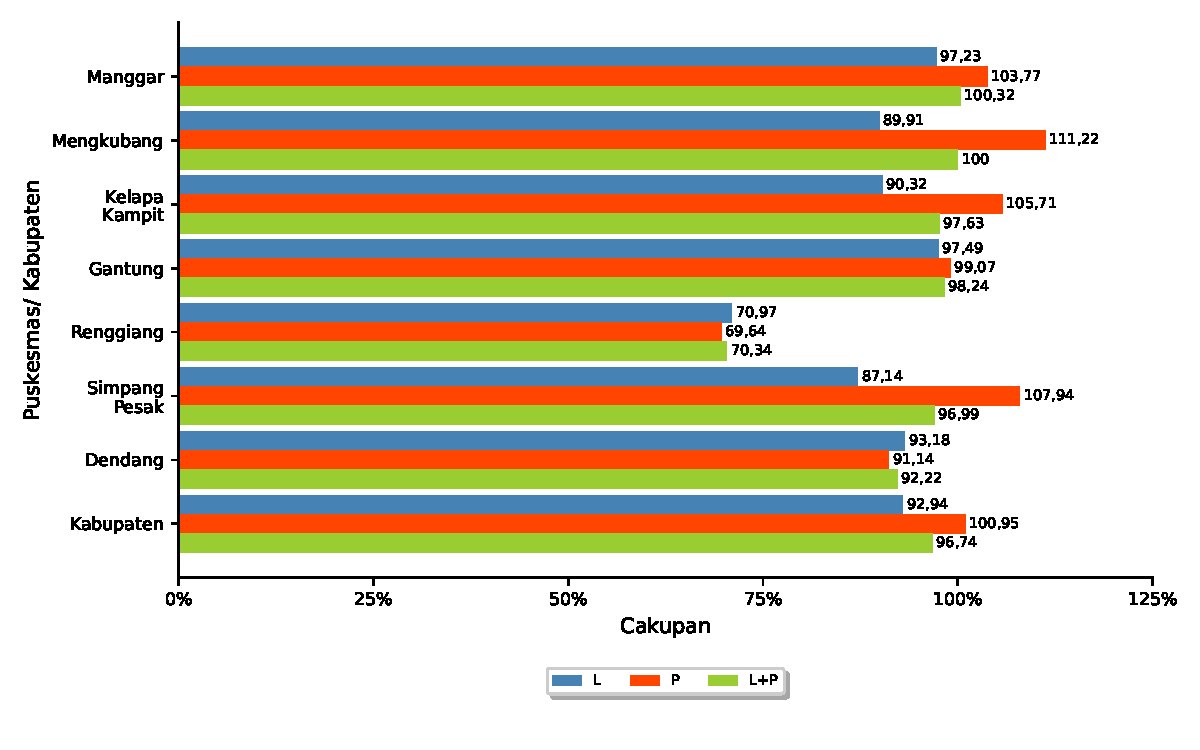
\includegraphics[width=0.85\textwidth]{bab_05/bab_05_16_pelayananBayi}
    \caption{Cakupan Pelayanan Kesehatan Bayi di Kab. Belitung Timur tahun \tP per Puskesmas}
    \label{fig:Cakupan-Pelayanan-Kesehatan-Bayi}
\end{figure}

\subsection{Cakupan Desa/ Kelurahan UCI}
Pencapaian \emph{Universal Child Immunization} (UCI) pada dasarnya merupakan
\emph{proxy} terhadap cakupan sasaran bayi yang telah mendapatkan imunisasi
secara lengkap. Desa/ kelurahan UCI adalah Desa/ kelurahan dimana
paling sedikit 80\% dari jumlah bayi yang ada di desa tersebut sudah
mendapat imunisasi dasar lengkap dalam waktu satu tahun.

Pada tahun \tP sebanyak 35 desa dari total 39 desa yang ada di Kabupaten Belitung
Timur telah mencapai UCI, sehingga capaian UCI Kabupaten Belitung
Timur pada tahun \tP adalah 89,74\% (\autoref{fig:Cakupan-Desa-UCI}).

\begin{figure}[H]
    \centering
    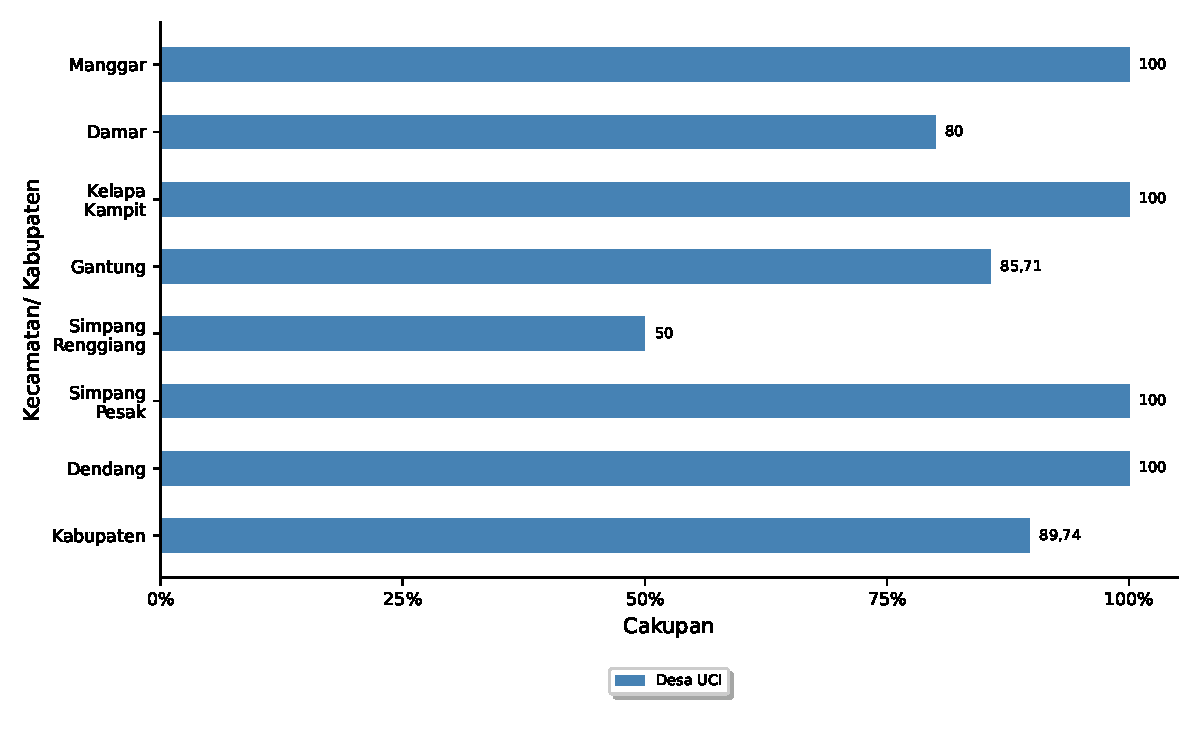
\includegraphics[width=0.85\textwidth]{bab_05/bab_05_17_UCI}
    \caption{Cakupan Desa/ Kelurahan UCI di Kab. Belitung Timur Tahun \tP per Puskesmas}
    \label{fig:Cakupan-Desa-UCI}
\end{figure}

\subsection{Imunisasi}
Imunisasi adalah upaya stimulasi terhadap sistem kekebalan tubuh untuk
menghasilkan antibodi dalam upaya melawan penyakit menular tertentu.
Program imunisasi melalui pemberian vaksin merangsang antibodi menggunakan
antigen yang telah dilemahkan yang berasal dari vaksin. Beberapa penyakit
menular yang termasuk ke dalam Penyakit yang Dapat Dicegah dengan
Imunisasi (PD3I) antara lain TBC, Difteri, Tetanus, Hepatitis B, Pertusis,
Campak, Polio, radang selaput otak, dan radang paru-paru.

\subsubsection{Imunisasi pada bayi}
Imunisasi dasar bayi meliputi pemberian imunisasi Hepatitis B pada
bayi usia 0-7 hari, imunisasi BCG pada bayi usia 0-11 bulan, imunisasi
Polio pada bayi usia 0-11 bulan dengan interval minimal 1 bulan, imunisasi
DPT-HB/DPT-HB-Hib pada bayi usia 2-11 bulan dengan interval minimal
1 bulan, dan imunisasi Campak pada bayi usia 9-11 bulan.

Cakupan imunisasi HB0 di Kabupaten Belitung Timur pada tahun \tP adalah sebesar 94,54\% (\autoref{fig:Cakupan-Imunisasi-HB0}), dan cakupan imunisasi BCG adalah 88,54\% (\autoref{fig:Cakupan-Imunisasi-BCG}).

Cakupan imunisasi DPT-HB-Hib3 di Kabupaten Belitung Timur pada tahun \tP
adalah sebesar 87,09\% (\autoref{fig:Cakupan-Imunisasi-DPT}), dan cakupan imunisasi Polio 4 adalah 87,24\% (\autoref{fig:Cakupan-Imunisasi-Polio4}).

Program imunisasi pada bayi bertujuan agar setiap bayi mendapatkan
imunisasi dasar secara lengkap. Bayi dikatakan mendapat imunisasi
dasar lengkap jika telah menerima 1 dosis imunisasi Hepatitis B, 1
dosis imunisasi BCG, 3 dosis imunisasi DPT-HB/DPT-HB-Hib, 4 dosis
imunisasi polio, dan 1 dosis imunisasi campak.

\begin{figure}[H]
    \centering
    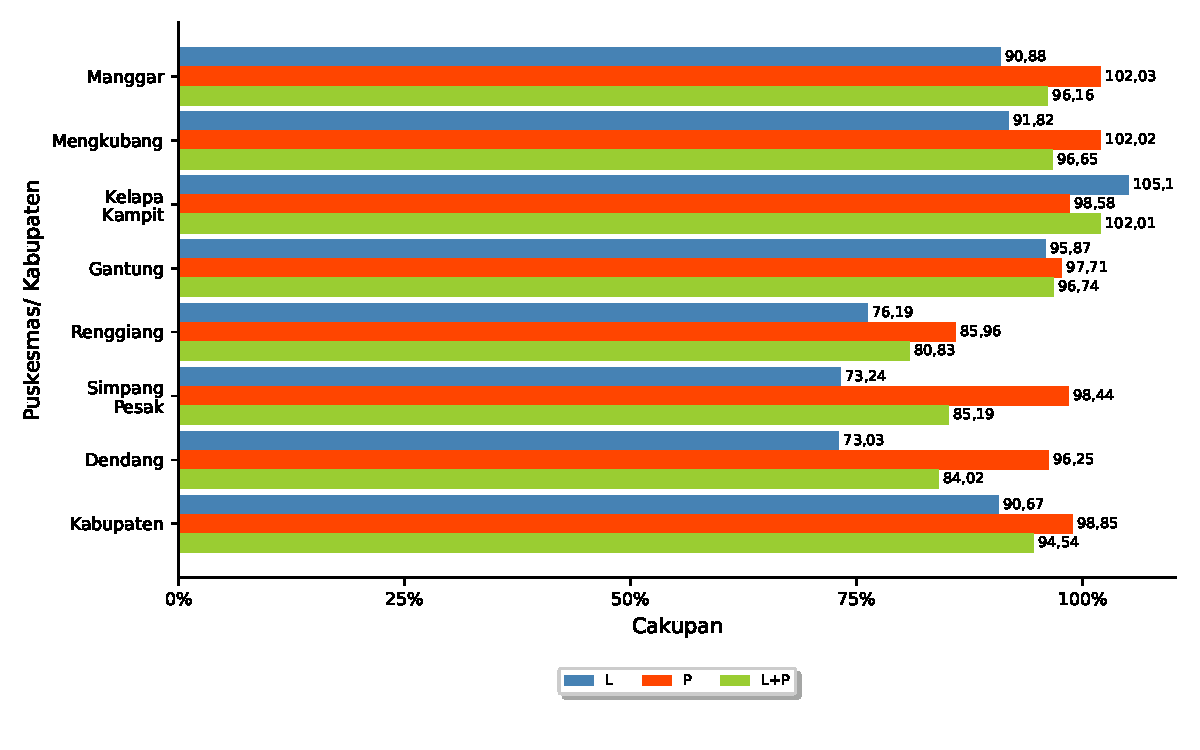
\includegraphics[width=0.85\textwidth]{bab_05/bab_05_18a_imunHB0}
    \caption{Cakupan Imunisasi HB0 di Kab. Belitung Timur Tahun \tP per Puskesmas}
    \label{fig:Cakupan-Imunisasi-HB0}
\end{figure}

\begin{figure}[H]
    \centering
    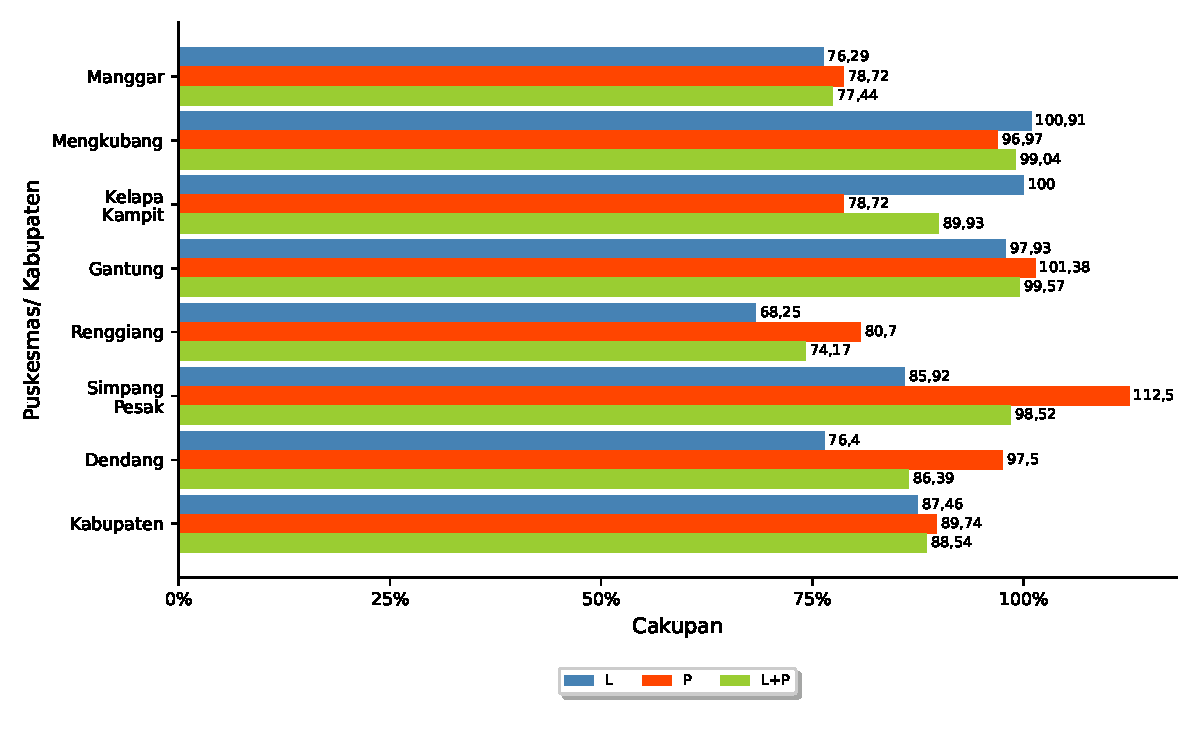
\includegraphics[width=0.85\textwidth]{bab_05/bab_05_18b_imunBCG}
    \caption{Cakupan Imunisasi BCG di Kab. Belitung Timur Tahun \tP per Puskesmas}
    \label{fig:Cakupan-Imunisasi-BCG}
\end{figure}

\begin{figure}[H]
    \centering
    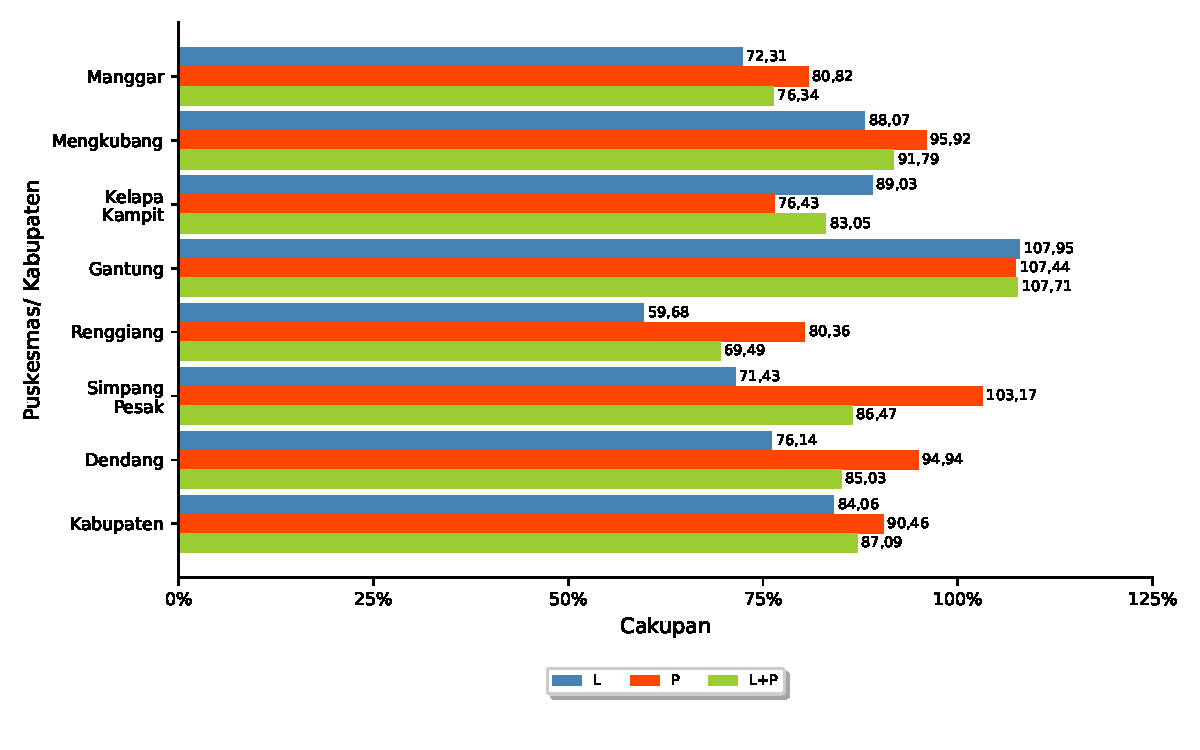
\includegraphics[width=0.85\textwidth]{bab_05/bab_05_19a_imunDPT}
    \caption{Cakupan Imunisasi DPT-HB-Hib3 di Kab. Belitung Timur Tahun \tP per Puskesmas}
    \label{fig:Cakupan-Imunisasi-DPT}
\end{figure}

\begin{figure}[H]
    \centering
    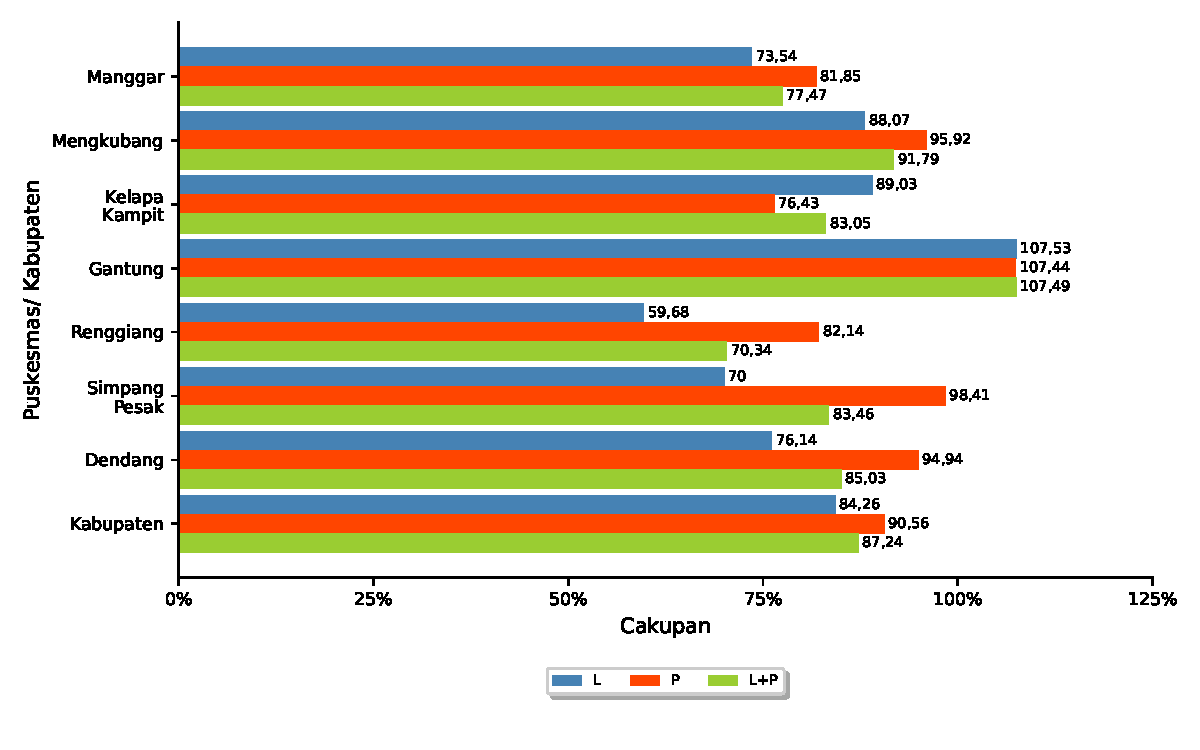
\includegraphics[width=0.85\textwidth]{bab_05/bab_05_19b_imunPol4}
    \caption{Cakupan Imunisasi Polio 4 di Kab. Belitung Timur Tahun \tP per Puskesmas}
    \label{fig:Cakupan-Imunisasi-Polio4}
\end{figure}

\begin{figure}[H]
    \centering
    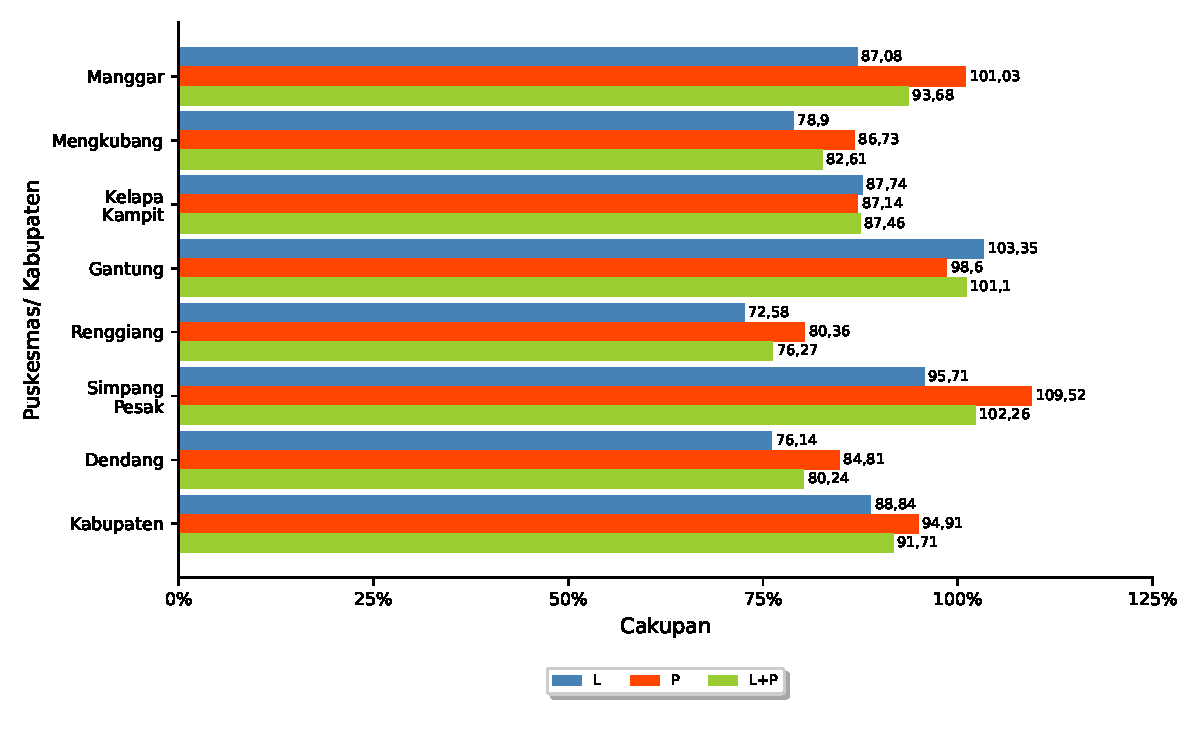
\includegraphics[width=0.85\textwidth]{bab_05/bab_05_20a_imunCampak}
    \caption{Cakupan Imunisasi Campak di Kab. Belitung Timur Tahun \tP per Puskesmas}
    \label{fig:Cakupan-Imunisasi-Campak}
\end{figure}

Cakupan imunisasi Campak di Kabupaten Belitung Timur pada tahun \tP adalah sebesar 91,71\% (\autoref{fig:Cakupan-Imunisasi-Campak}).
%menurun dari cakupan tahun 2019 sebesar 92,03\%.

Cakupan imunisasi dasar lengkap (IDL) di Kabupaten Belitung Timur pada tahun \tP adalah sebesar 92,77\% (\autoref{fig:Cakupan-Imunisasi-IDL}).

\begin{figure}[H]
    \centering
    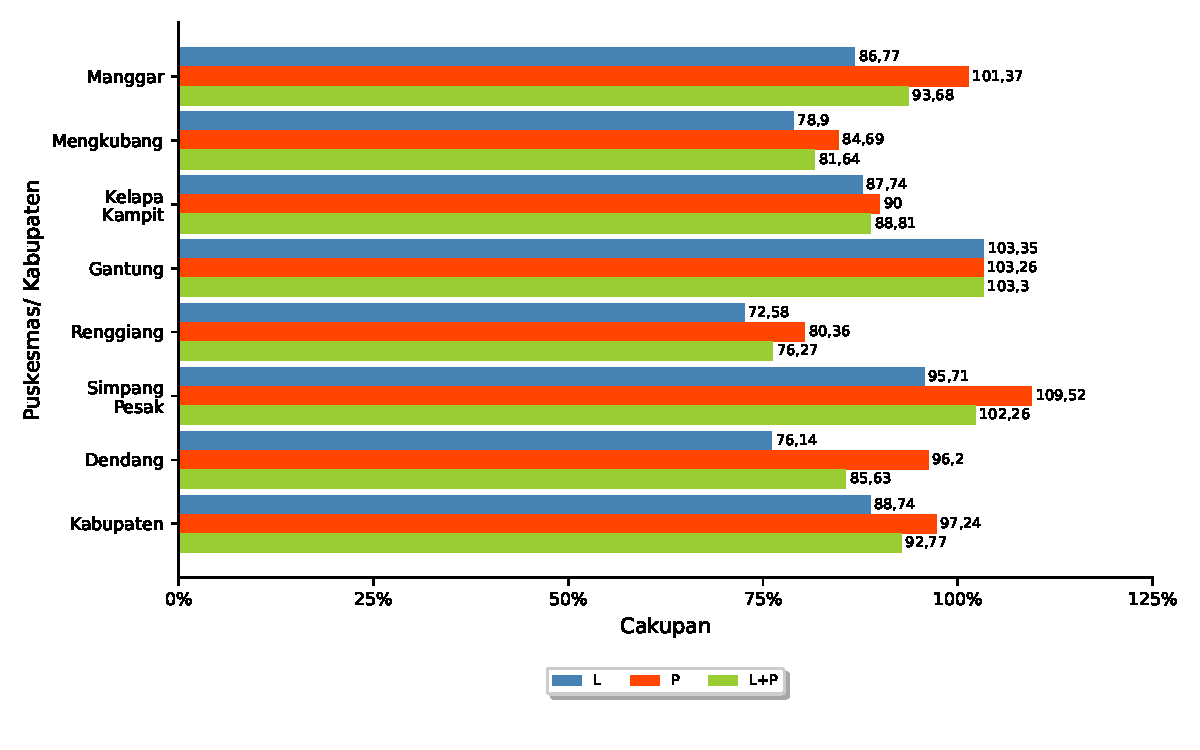
\includegraphics[width=0.85\textwidth]{bab_05/bab_05_20b_imunIDL}
    \caption{Cakupan Imunisasi Dasar Lengkap di Kab. Belitung Timur Tahun \tP per Puskesmas}
    \label{fig:Cakupan-Imunisasi-IDL}
\end{figure}

\subsubsection{Imunisasi pada balita}
Imunisasi lanjutan diperlukan untuk mempertahankan tingkat kekebalan yang optimal pada anak.
Imunisasi lanjutan meliputi pemberian imunisasi DPT-HB-Hib 4 pada anak usia 12-24 bulan serta imunisasi Campak 2 pada anak usia 12-24 bulan.

Cakupan imunisasi DPT-HB-Hib 4 di Kabupaten Belitung Timur pada tahun \tP
adalah sebesar 72,79\% (\autoref{fig:Cakupan-Imunisasi-DPT4}), sedangkan cakupan imunisasi Campak 2 adalah 73,34\% (\autoref{fig:Cakupan-Imunisasi-Campak2}).

\begin{figure}[H]
    \centering
    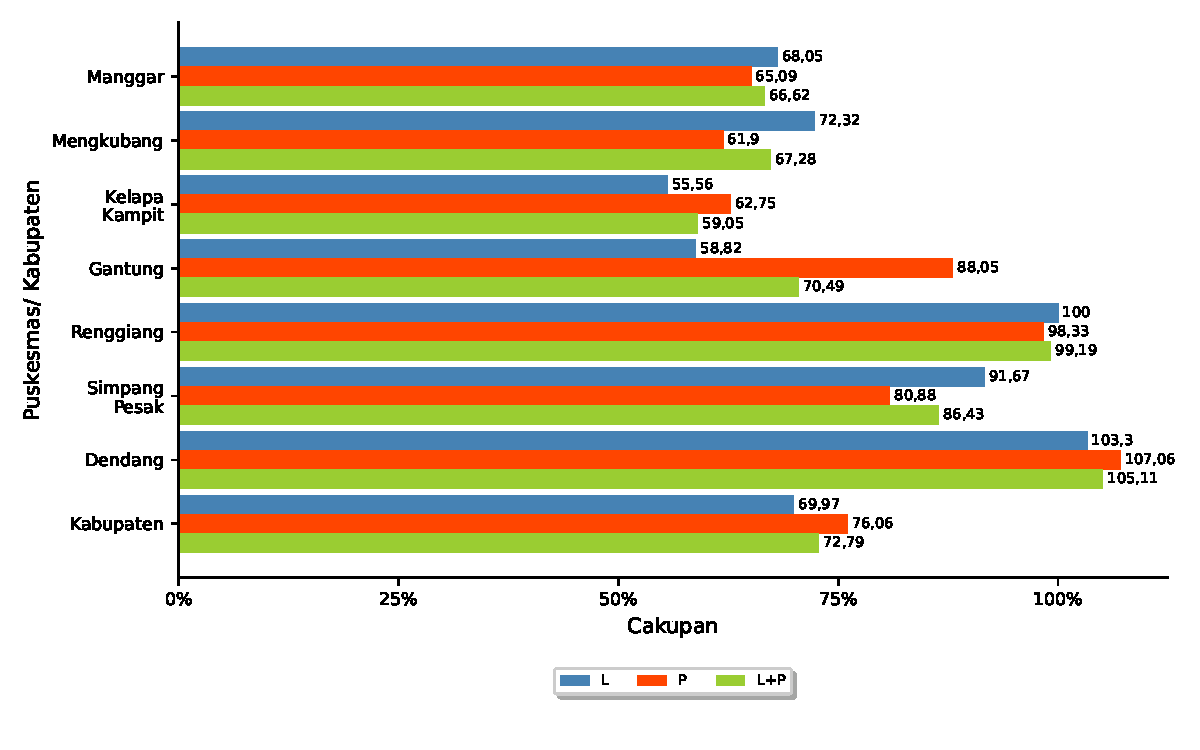
\includegraphics[width=0.85\textwidth]{bab_05/bab_05_21a_imunDPTlanjut}
    \caption{Cakupan Imunisasi DPT-HB-Hib 4 di Kab. Belitung Timur Tahun \tP per Puskesmas}
    \label{fig:Cakupan-Imunisasi-DPT4}
\end{figure}

\begin{figure}[H]
    \centering
    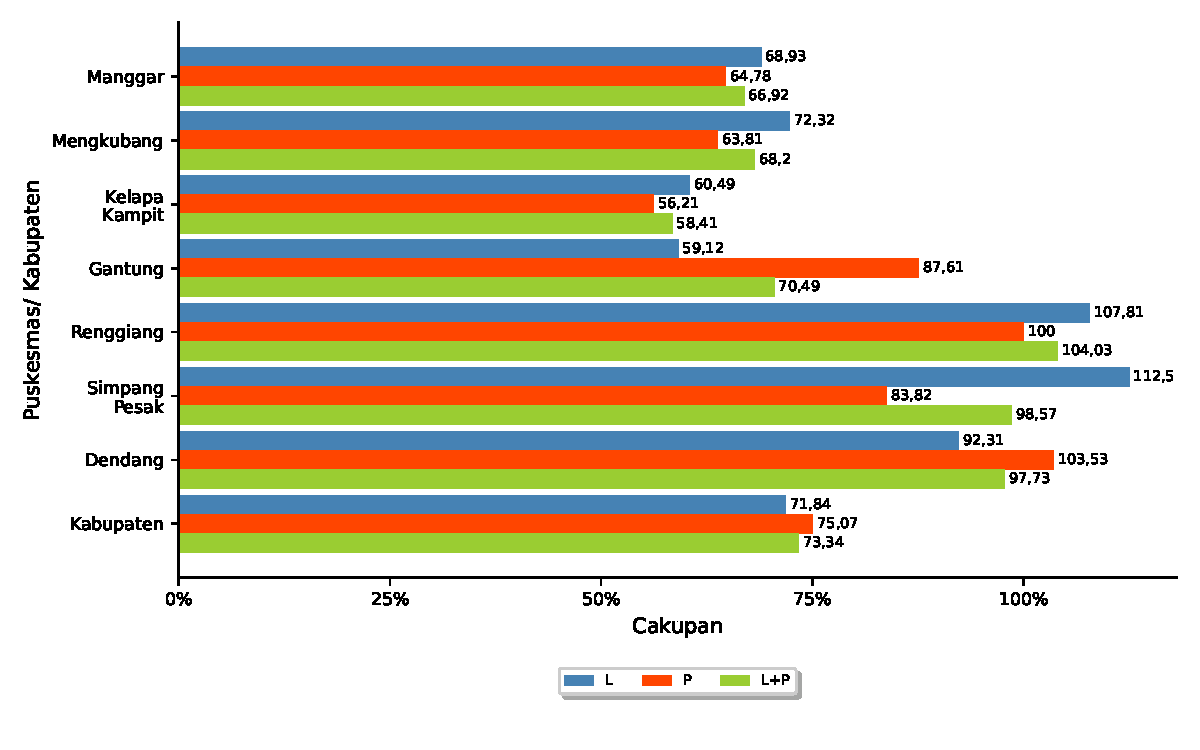
\includegraphics[width=0.85\textwidth]{bab_05/bab_05_21b_imunCampakLanjut}
    \caption{Cakupan Imunisasi Campak 2 di Kab. Belitung Timur Tahun \tP per Puskesmas}
    \label{fig:Cakupan-Imunisasi-Campak2}
\end{figure}

\subsection{Pemberian Kapsul Vitamin A}
Upaya perbaikan gizi juga dilakukan kepada beberapa sasaran yang diperkirakan
banyak mengalami kekurangan Vitamin A. Vitamin A adalah salah satu
zat gizi penting yang larut dalam lemak, disimpan dalam hati, dan
tidak dapat diproduksi oleh tubuh sehingga harus dipenuhi dari luar
tubuh. Kekurangan Vitamin A (KVA) dapat menurunkan sistem kekebalan
tubuh balita serta meningkatkan risiko kesakitan dan kematian. Kekurangan
Vitamin A juga merupakan penyebab utama kebutaan pada anak yang dapat
dicegah.

Pemberian Vitamin A dilakukan berupa pemberian kapsul vitamin A biru 100.000 IU bagi bayi
usia enam sampai dengan sebelas bulan, dan kapsul vitamin A merah 200.000
IU untuk anak balita usia dua belas sampai dengan lima puluh sembilan sebanyak
bulan.

Cakupan pemberian vitamin A pada balita usia 6-59 tahun pada tahun \tP di Kabupaten Belitung Timur adalah 86,60\% (\autoref{fig:Cakupan-Vitamin-A-Balita}).
% meningkat dari cakupan tahun 2021 sebesar 81,47\%.

\begin{figure}[H]
    \centering
    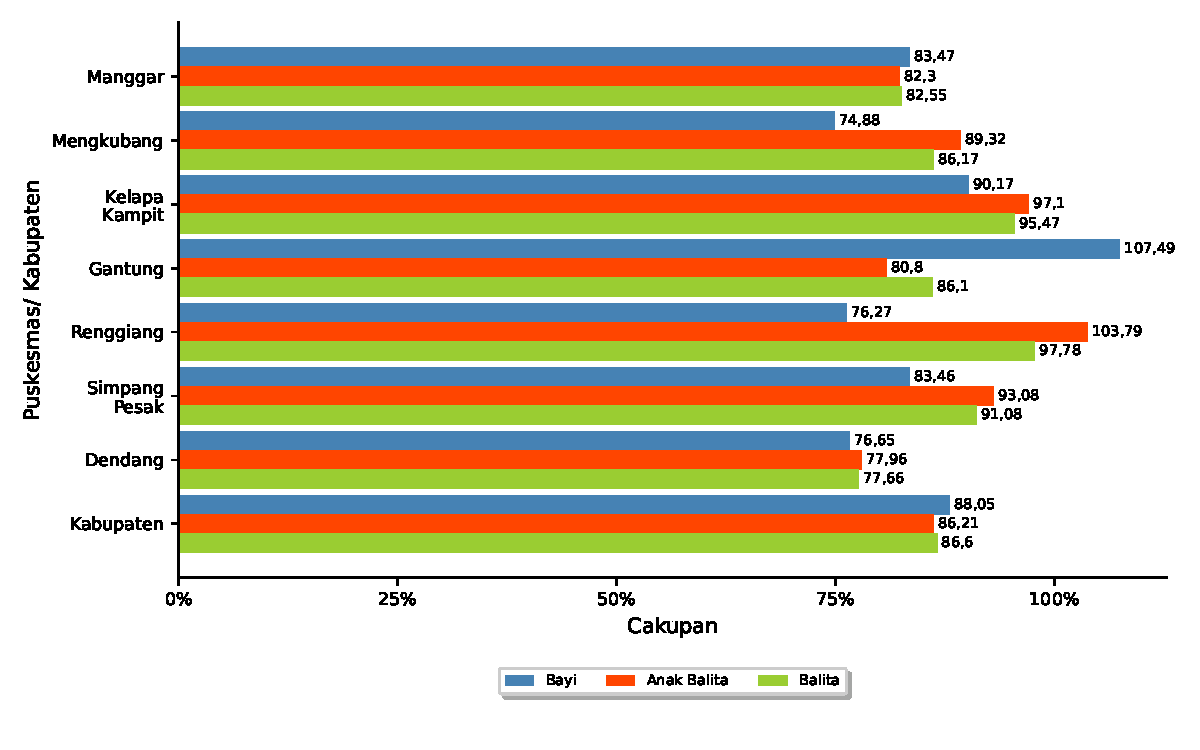
\includegraphics[width=0.9\textwidth]{bab_05/bab_05_22_bayiBalitaVitA}
    \caption{Cakupan Pemberian Vitamin A Balita 6-59 Bulan di Kab. Belitung Timur Tahun \tP per Puskesmas}
    \label{fig:Cakupan-Vitamin-A-Balita}
\end{figure}


\subsection{Pelayanan Kesehatan Anak Balita}
Pelayanan kesehatan anak balita mencakup pemantauan tumbuh kembang dan pelayanan Stimulasi Deteksi dan Intervensi Dini Tumbuh Kembang (SDIDTK).
Balita yang dipantau tumbuh kembang adalah  balita yang ditimbang sedikitnya 8 kali dalam satu tahun, diukur panjang badan atau tinggi badannya sedikitnya 2 kali dalam satu tahun dan dipantau perkembangan sedikitnya 2 kali dalam satutahun. Pemantauan perkembangan menggunakan ceklis Buku KIA atau KPSP atau instrument baku lainnya.
Balita dilayani SDIDTK adalah balita yang dipantau tahapan perkembangan sesuai usianya (usia 0-24 bulan: 3 bulan sekali; usia 24-72 bulan: 6 bulan sekali) menggunakan instrument dalam SDIDTK oleh tenaga kesehatan dalam kurun waktu 1 tahun.

Cakupan balita dipantau tumbuh kembang di Kabupaten Belitung Timur pada tahun \tP adalah sebesar 99,01\%, sedangkan cakupan balita dilayani SDIDTK di Kabupaten Belitung Timur pada tahun \tP adalah sebesar 82,52\%. (\autoref{fig:Cakupan-Pelayanan-Balita-Tumbuh-Kembang}).

\begin{figure}[H]
	\centering
	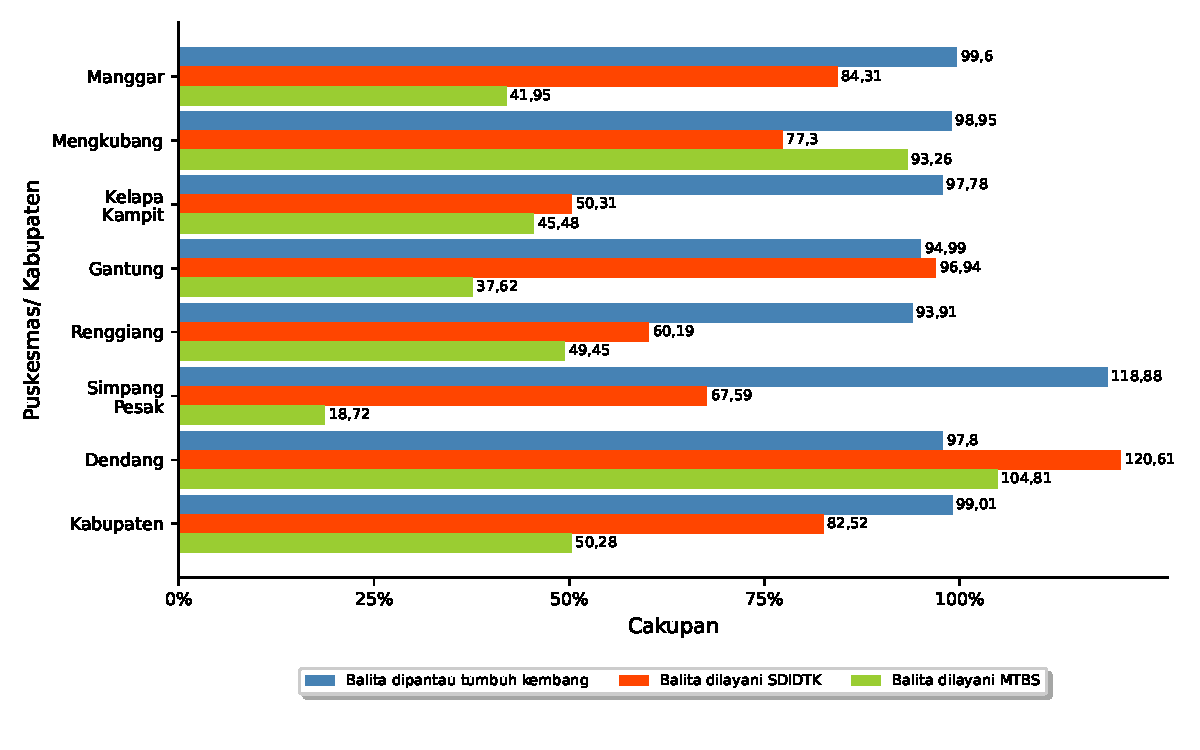
\includegraphics[width=0.85\textwidth]{bab_05/bab_05_23_balitaTumbuhKembang}
	\caption{Cakupan Balita Dipantau Tumbuh Kembang di Kab. Belitung Timur tahun \tP per Puskesmas}
	\label{fig:Cakupan-Pelayanan-Balita-Tumbuh-Kembang}
\end{figure}

\subsection{Balita Ditimbang}
\label{subsec:Balita-Ditimbang}
Peran serta masyarakat dalam penimbangan balita menjadi sangat penting
dalam deteksi dini kasus gizi kurang dan gizi buruk. Dengan rajin
menimbang balita, maka pertumbuhan balita dapat dipantau secara intensif.
Sehingga bila berat badan anak tidak naik ataupun jika ditemukan penyakit
akan dapat segera dilakukan upaya pemulihan dan pencegahan supaya
tidak menjadi gizi kurang atau gizi buruk. Semakin cepat ditemukan,
maka penanganan kasus gizi kurang atau gizi buruk akan semakin baik.\par

Cakupan penimbangan balita di posyandu (D/S) adalah jumlah balita
yang ditimbang di seluruh posyandu yang melapor di satu wilayah kerja
pada kurun waktu tertentu dibagi jumlah seluruh balita yang ada di
seluruh posyandu yang melapor di satu wilayah kerja pada kurun waktu
tertentu.

Cakupan balita ditimbang di Kabupaten Belitung Timur pada tahun \tP yaitu sebesar 43,92\% (\autoref{fig:Cakupan-Balita-Ditimbang}), %meningkat dari cakupan tahun 2020 sebesar 57,91\%.

\begin{figure}[H]
  \centering
  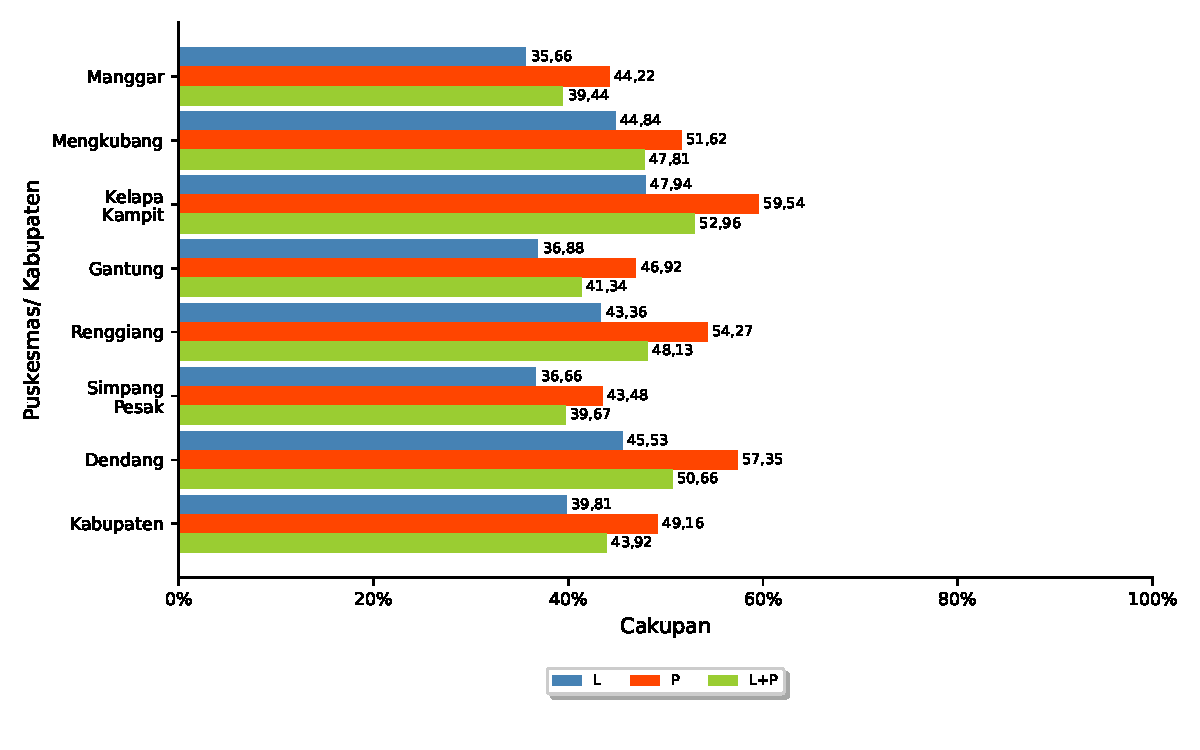
\includegraphics[width=0.85\textwidth]{bab_05/bab_05_24_balitaDitimbang}
  \caption{Cakupan Balita Ditimbang di Kab. Belitung Timur Tahun \tP per Puskesmas}
  \label{fig:Cakupan-Balita-Ditimbang}
\end{figure}


\subsection{Penemuan Kasus Balita Gizi Kurang, Balita Pendek, dan Balita Kurus}
\label{subsec:Penemuan-Kasus-Gizi-Kurang}
Balita Berat Badan Kurang adalah balita dengan status gizi yang didasarkan pada indeks berat badan menurut umur (BB/U) yang merupakan gabungan dari istilah gizi buruk dan gizi kurang dengan Z score < -2 standar deviasi, di mana Z score adalah nilai simpangan berat badan atau tinggi badan dari nilai berat badan atau tinggi badan normal menurut baku pertumbuhan WHO.
Balita Pendek adalah balita dengan status gizi yang didasarkan pada indeks panjang badan menurut umur (PB/U) atau tinggi badan menurut umur (TB/U) dengan Z score < -2 standar deviasi.
Balita Gizi Kurang adalah balita dengan status gizi yang didasarkan pada indeks berat badan menurut panjang badan (BB/PB) atau berat badan menurut tinggi badan (BB/TB) dengan Z score -2 hingga -3 standar deviasi.
Balita Gizi Buruk adalah balita dengan status gizi yang didasarkan pada indeks berat badan menurut panjang badan (BB/PB) atau berat badan menurut tinggi badan (BB/TB) dengan Z score < -3 standar deviasi.

\begin{figure}[H]
  \centering
  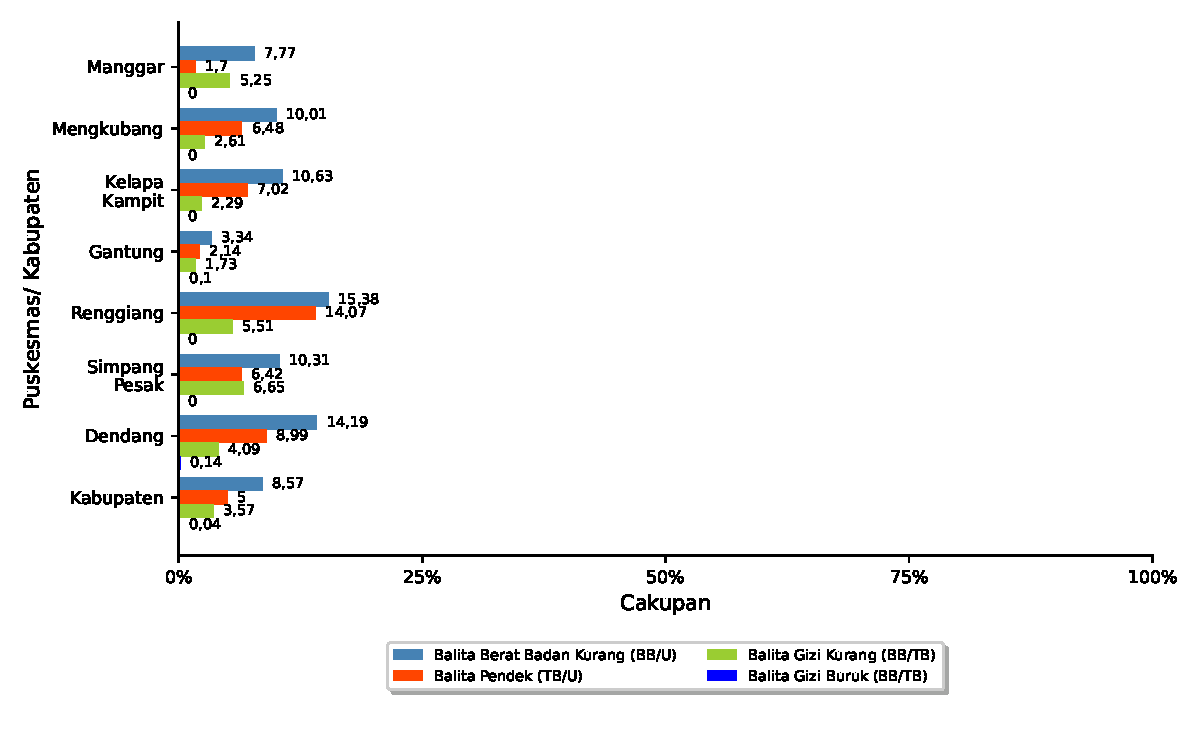
\includegraphics[width=0.85\textwidth]{bab_05/bab_05_25_statusGiziBalita}
  \caption{Sebaran Status Gizi Balita Berdasarkan Indeks BB/U, TB/U, dan BB/TB di Kab. Belitung Timur Tahun \tP per
Puskesmas}
  \label{fig:Status-Gizi-Balita}
\end{figure}

Pada tahun \tP, tercatat bahwa kasus Balita Berat Badan Kurang (BB/U) berjumlah 618 kasus atau 8,57\% dari jumlah balita ditimbang.
Kasus Balita Pendek (TB/U) atau \textit{stunting} berjumlah 360 kasus atau 5,00\% dari jumlah balita ditimbang.
Kasus Balita Gizi Kurang (BB/TB) berjumlah 256 kasus atau 3,57 \% dari jumlah balita ditimbang.
Kasus Balita Gizi Buruk (BB/TB) berjumlah 3 kasus atau 0,04 \% dari jumlah balita ditimbang (\autoref{fig:Status-Gizi-Balita}).

\subsection{Penjaringan Kesehatan Siswa SD, SMP, SMA}
Penjaringan kesehatan siswa SD/ MI adalah pemeriksaan kesehatan umum terhadap murid kelas 1 SD, MI atau setingkat yang dilaksanakan oleh tenaga kesehatan bersama kader kesehatan sekolah yang mencakup minimal pemeriksaan status gizi (TB,BB), pemeriksaan gigi, tajam penglihatan dan tajam pendengaran di satu wilayah kerja pada kurun waktu tertentu.

Cakupan penjaringan kesehatan siswa SD/ MI di Kabupaten Belitung Timur pada tahun \tP adalah sebesar 100,00\%.

Penjaringan kesehatan siswa SMP dan setingkat adalah pemeriksaan kesehatan umum terhadap murid kelas 7 SMP, MTs atau setingkat yang dilaksanakan oleh tenaga kesehatan bersama kader kesehatan sekolah yang mencakup minimal pemeriksaan status gizi (TB,BB), pemeriksaan gigi, tajam penglihatan dan tajam pendengaran di satu wilayah kerja pada kurun waktu tertentu.

Cakupan penjaringan kesehatan siswa SMP/ MTs di Kabupaten Belitung Timur pada tahun \tP adalah sebesar 100,00\%.

Penjaringan kesehatan siswa SMA/ MA adalah pemeriksaan kesehatan umum terhadap murid kelas 10 SMA, MA atau setingkat yang dilaksanakan oleh tenaga kesehatan bersama kader kesehatan sekolah yang mencakup minimal pemeriksaan status gizi (TB,BB), pemeriksaan gigi, tajam penglihatan dan tajam pendengaran di satu wilayah kerja pada kurun waktu tertentu.

Cakupan penjaringan kesehatan siswa SMA/ MA di Kabupaten Belitung Timur pada tahun \tP adalah sebesar 100,00\%.

\begin{figure}[H]
    \centering
    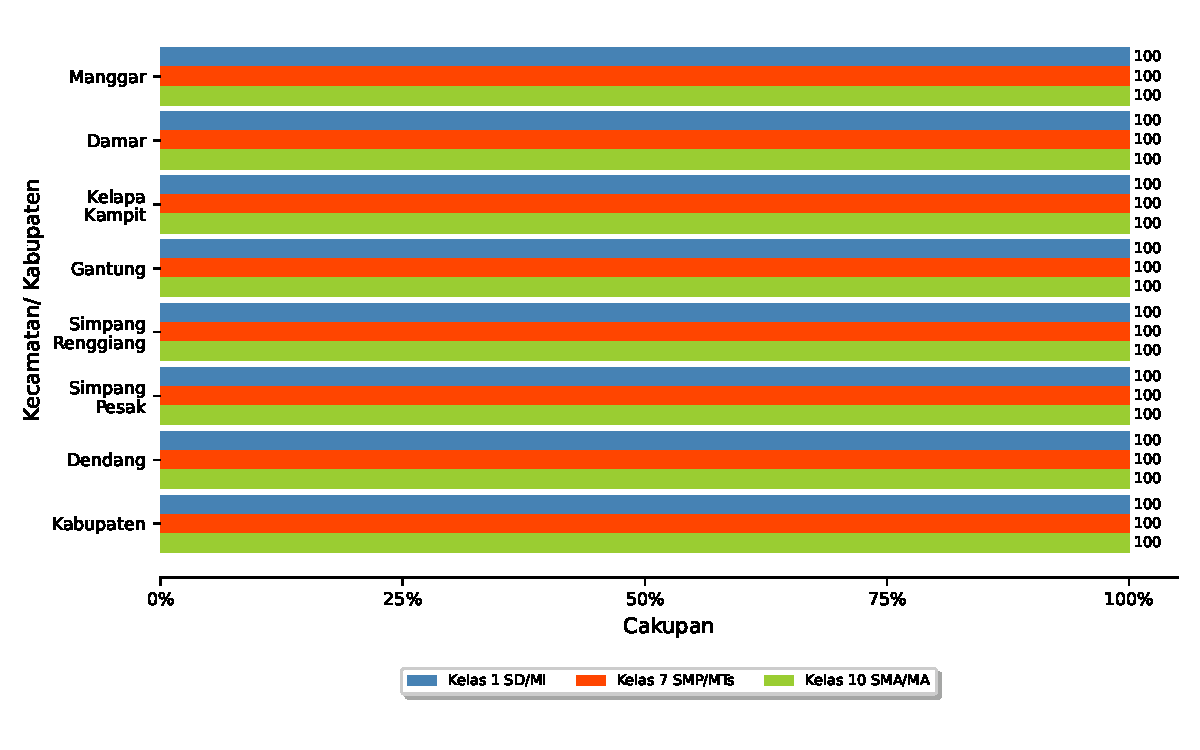
\includegraphics[width=0.85\textwidth]{bab_05/bab_05_26_kesehatanSiswa}
    \caption{Cakupan Penjaringan Kesehatan Siswa SD/ MI, SMP/ MTs, SMA/ MA di Kab. Belitung Timur Tahun \tP per Kecamatan}
    \label{fig:Cakupan-Penjaringan-Siswa}
\end{figure}

Pelayanan kesehatan usia pendidikan dasar sesuai standar meliputi :
\begin{enumerate}
    \item Skrining kesehatan.
    \item Tindaklanjut hasil skrining kesehatan.
\end{enumerate}
yang dilakukan pada anak kelas 1 sampai dengan kelas 9 di sekolah minimal satu kali dalam satu tahun ajaran dan usia 7 sampai 15 tahun diluar sekolah.

Cakupan pelayanan kesehatan usia pendidikan dasar di Kabupaten Belitung Timur pada tahun \tP adalah sebesar 99,96\% (\autoref{fig:Cakupan-Pelayanan-Kesehatan-Usia-Dikdas}).

\begin{figure}[H]
    \centering
    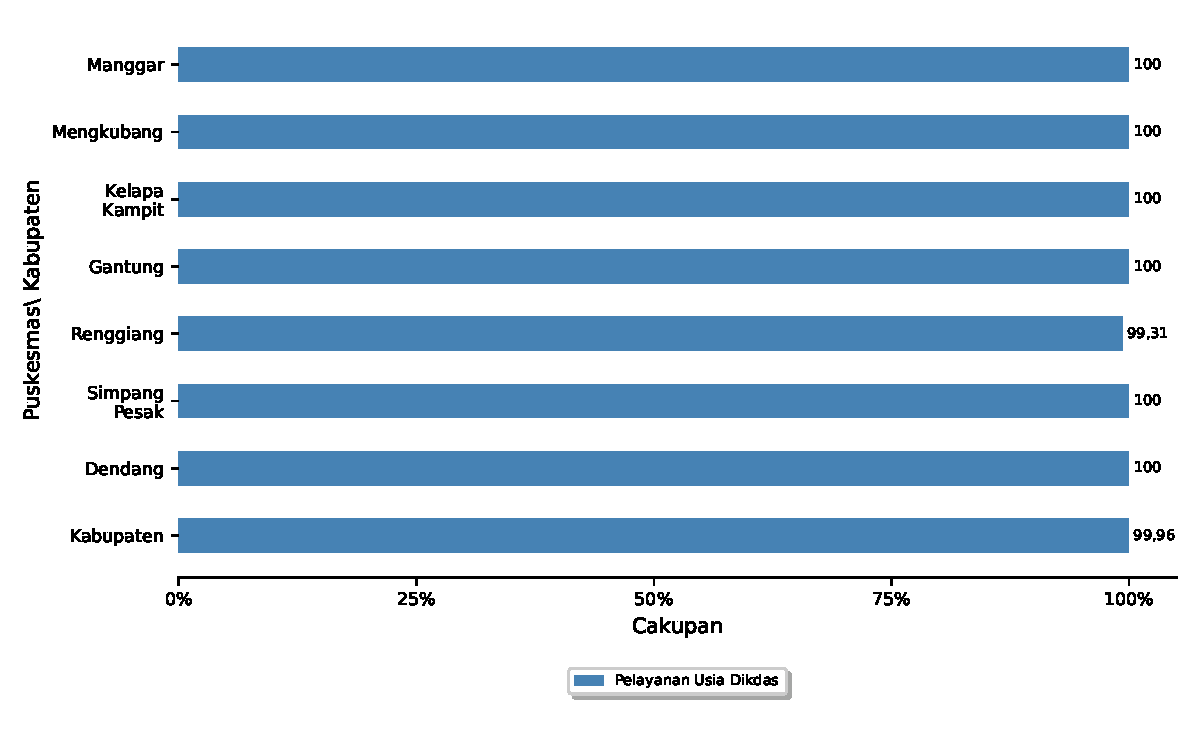
\includegraphics[width=0.85\textwidth]{bab_05/bab_05_26_kesehatanSiswa_spm}
    \caption{Cakupan Pelayanan Kesehatan Usia Pendidikan Dasar di Kab. Belitung Timur Tahun \tP per Kecamatan}
    \label{fig:Cakupan-Pelayanan-Kesehatan-Usia-Dikdas}
\end{figure}

\section{KESEHATAN GIGI DAN MULUT}
\subsection{Pelayanan Kesehatan Gigi dan Mulut}
Setiap penyelenggaraan upaya kesehatan gigi dan mulut yang dilakukan untuk meningkatkan kesehatan gigi dan mulut, mencegah dan menyembuhkan penyakit serta memulihkan kesehatan gigi dan mulut perorangan, keluarga, kelompok atau masyarakat secara paripurna, terpadu dan berkualitas.
Pelayanan kesehatan gigi dan mulut yang diberikan dapat berupa pemeriksaan, pengobatan, pencabutan gigi tetap/gigi sulung, penambalan tetap/sementara, perawatan pulpa, pembersihan karang gigi dan pembuatan gigi tiruan lepasan.

Rasio tumpatan/pencabutan adalah rasio jumlah penambalan gigi tetap terhadap jumlah pencabutan gigi tetap dalam setahun.
Cakupan kasus gigi dan mulut dirujuk adalah persentase kasus gigi dan mulut yang dikirim dari Puskesmas ke fasilitas kesehatan rujukan tingkat lanjut dalam satu tahun terhadap jumlah kunjungan baru dan lama rawat jalan gigi dan mulut di puskesmas meliputi pemeriksaan, pengobatan dan perawatan gigi dan mulut dalam satu tahun.

Rasio tumpatan/pencabutan di Kabupaten Belitung Timur pada tahun \tP adalah sebesar 0,99 (\autoref{fig:Cakupan-Pelayanan-Kesehatan-Gigi-Mulut-Tumpatan}).

\begin{figure}[H]
	\centering
	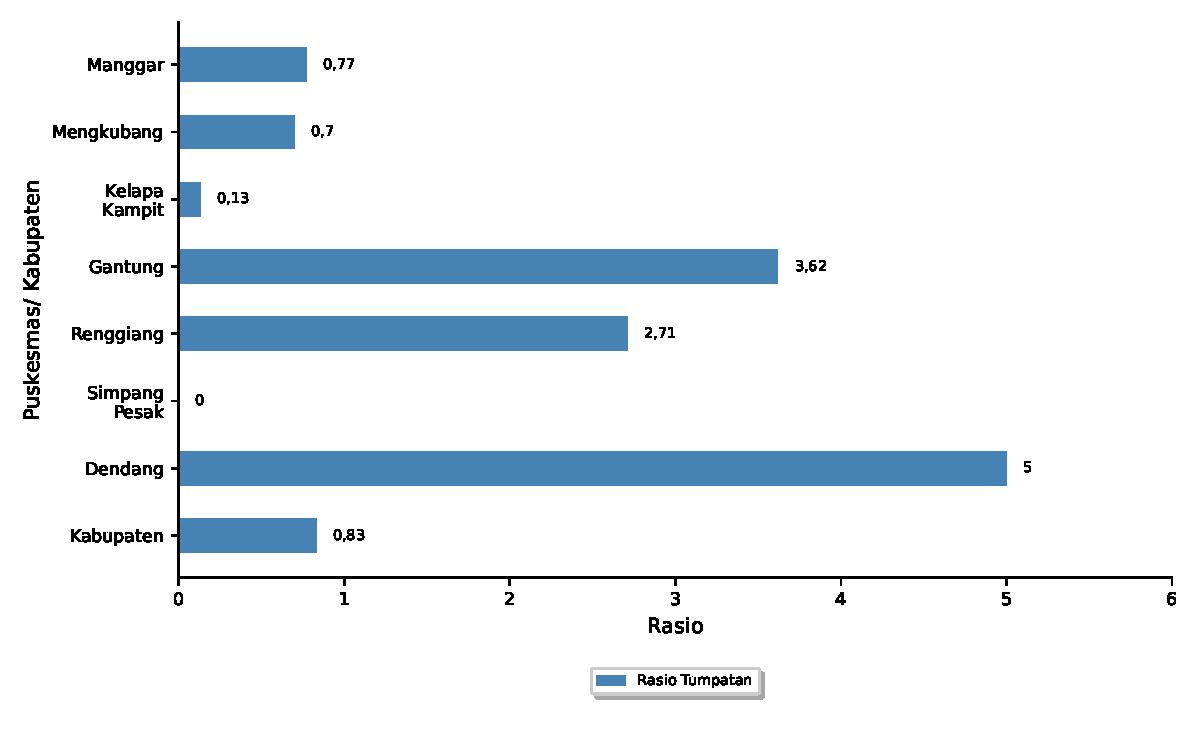
\includegraphics[width=0.85\textwidth]{bab_05/bab_05_27a_gimulTumpatan}
	\caption{Rasio Tumpatan/Pencabutan di Kab. Belitung Timur Tahun \tP per Puskesmas}
	\label{fig:Cakupan-Pelayanan-Kesehatan-Gigi-Mulut-Tumpatan}
\end{figure}

Cakupan kasus gigi dan mulut dirujuk di Kabupaten Belitung Timur pada tahun \tP adalah sebesar 6,51\% (\autoref{fig:Cakupan-Pelayanan-Kesehatan-Gigi-Mulut-Dirujuk}).

\begin{figure}[H]
	\centering
    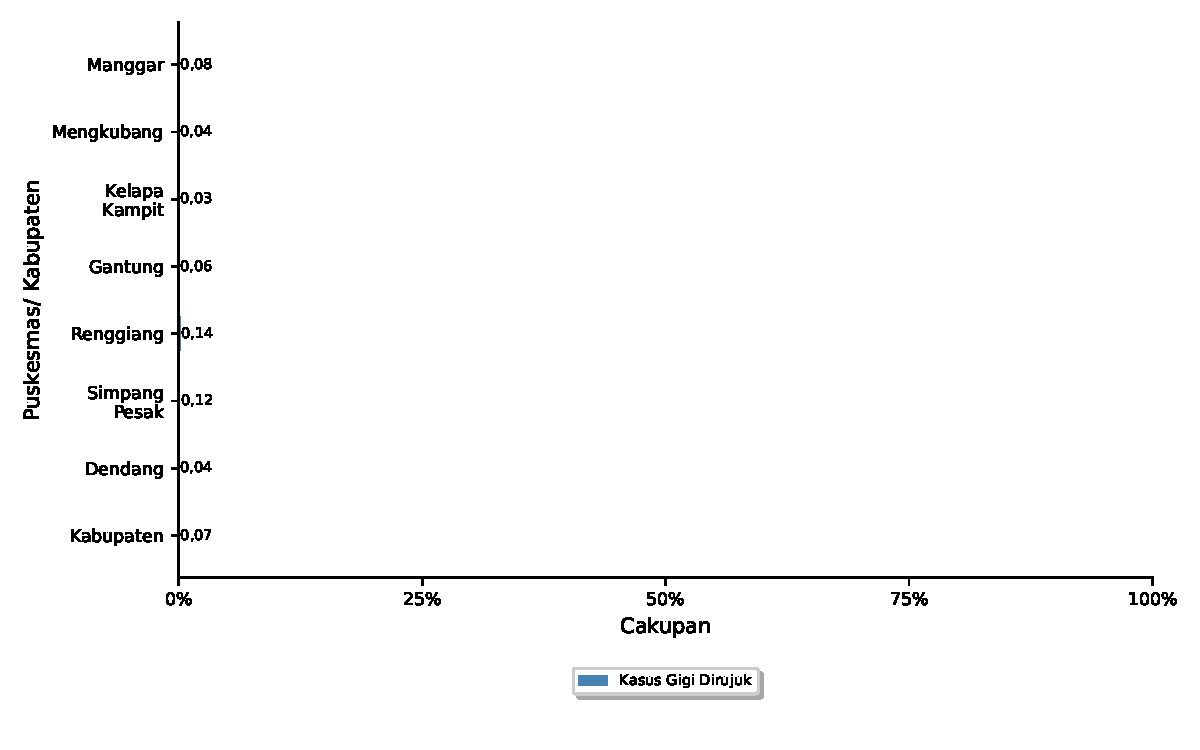
\includegraphics[width=0.85\textwidth]{bab_05/bab_05_27b_gimulDirujuk}
	\caption{Cakupan Kasus Gigi dan Mulut Dirujuk di Kab. Belitung Timur Tahun \tP per Puskesmas}
	\label{fig:Cakupan-Pelayanan-Kesehatan-Gigi-Mulut-Dirujuk}
\end{figure}

\subsection{Upaya Kesehatan Gigi Sekolah}
Penyelenggaraan upaya kesehatan gigi dan mulut anak sekolah tingkat dasar (SD/MI) atau UKGS dilakukan dengan mengutamakan pendekatan promotif dan preventif tanpa mengabaikan pendekatan kuratif dan rehabilitatif.
Perawatan kesehatan gigi dan mulut diberikan kepada murid SD/MI dalam bentuk preventif (\textit{topical fluoride}, \textit{surface protection}/\textit{fissure sealent} atau \textit{atraumatic restoration treatment}) dan kuratif sederhana seperti pengobatan, penambalan gigi, dan pencabutan gigi sulung maupun tetap yang dilakukan baik di sekolah maupun Puskesmas.

Cakupan pemeriksaan gigi dan mulut pada murid SD/MI di Kabupaten Belitung Timur pada tahun \tP adalah sebesar 89,83\% (\autoref{fig:Cakupan-Pelayanan-Kesehatan-Gigi-Mulut-SD}).

\begin{figure}[H]
	\centering
	\includegraphics[width=0.85\textwidth]{bab_05/bab_05_27c_gimulSDdiperiksa}
	\caption{Cakupan Pemeriksaan Gigi dan Mulut Murid SD/MI di Kab. Belitung Timur Tahun \tP per Puskesmas}
	\label{fig:Cakupan-Pelayanan-Kesehatan-Gigi-Mulut-SD}
\end{figure}

Cakupan perawatan gigi dan mulut pada murid SD/MI di Kabupaten Belitung Timur pada tahun \tP adalah sebesar 59,04\% (\autoref{fig:Cakupan-Pelayanan-Kesehatan-Gigi-Mulut-SD-Dirawat}).

\begin{figure}[H]
	\centering
	\includegraphics[width=0.85\textwidth]{bab_05/bab_05_27d_gimulSDdirawat}
	\caption{Cakupan Perawatan Gigi dan Mulut Murid SD/MI di Kab. Belitung Timur Tahun \tP per Puskesmas}
	\label{fig:Cakupan-Pelayanan-Kesehatan-Gigi-Mulut-SD-Dirawat}
\end{figure}

\section[USIPRO DAN USILA]{KESEHATAN USIA PRODUKTIF DAN USIA LANJUT}
\subsection{Pelayanan Kesehatan Usia Produktif}
Cakupan pelayanan kesehatan usia produktif adalah cakupan penduduk usia 15–59 tahun yang mendapat pelayanan skrining kesehatan sesuai standar di wilayah kerjanya dalam kurun waktu satu tahun. Edukasi dilaksanakan di Fasilitas Pelayanan Kesehatan dan/ atau UKBM dan/ atau kunjungan rumah. Pelayanan kesehatan sesuai standar meliputi:
\begin{enumerate}
  \item Edukasi kesehatan termasuk keluarga berencana;
  \item Skrining faktor risiko penyakit menular dan penyakit tidak menular:
  \begin{enumerate}
    \item Pengukuran tinggi badan, berat badan, dan lingkar perut;
    \item Pengukuran tekanan darah;
    \item Pemeriksaan gula darah; dan
    \item Anamnesa perilaku berisiko.
  \end{enumerate}
\end{enumerate}

Cakupan pelayanan kesehatan usia produktif di Kabupaten Belitung Timur pada tahun \tP adalah 88,49\% (\autoref{fig:Cakupan-Yankes-Usprod}).
%, meningkat dari cakupan tahun 2021 sebesar 65,23\%.
Dari 74.911 orang penduduk yang diskrining, sebanyak 15.166 orang (20,25\%) ditemukan beresiko PTM (\autoref{fig:Cakupan-Resiko-PTM-Usprod}).

\begin{figure}[H]
    \centering
    \includegraphics[width=0.85\textwidth]{bab_05/bab_05_28_skriningProduktif_a}
    \caption{Cakupan Pelayanan Kesehatan Usia Produktif di Kab. Belitung Timur Tahun \tP per Puskesmas}
    \label{fig:Cakupan-Yankes-Usprod}
\end{figure}

\begin{figure}[H]
    \centering
    \includegraphics[width=0.85\textwidth]{bab_05/bab_05_28_skriningProduktif_b}
    \caption{Penemuan Resiko PTM Usia Produktif di Kab. Belitung Timur Tahun \tP per Puskesmas}
    \label{fig:Cakupan-Resiko-PTM-Usprod}
\end{figure}

\subsection{Pelayanan Kesehatan Calon Pengantin}
Calon pengantin (catin) merupakan kelompok sasasan yang perlu mendapatkan intervensi dalam pelayanan kesehatan reproduksi.
Pemberian KIE kesehatan reproduksi kepada calon pengantin merupakan salah satu upaya strategis untuk meningkatkan derajat kesehatan ibu dan bayi baru lahir melalui peningkatan pengetahuan calon pengantin agar kelak dapat merencanakan kehamilan yang sehat dan melahirkan generasi penerus yang berkualitas.

Cakupan pelayanan kesehatan calon pengantin di Kabupaten Belitung Timur pada tahun \tP adalah 97,84\% (\autoref{fig:Cakupan-Yankes-Catin}).

\begin{figure}[H]
	\centering
	\includegraphics[width=0.85\textwidth]{bab_05/bab_05_29a_pelayananCatin}
	\caption{Cakupan Pelayanan Kesehatan Calon Pengantin di Kab. Belitung Timur Tahun \tP per Puskesmas}
	\label{fig:Cakupan-Yankes-Catin}
\end{figure}

Dari 905 catin perempuan yang diperiksa ditemukan 209 orang (23,09\%) yang mengidap anemia dan 157 orang (17,35\%) yang mengalami gizi kurang.

\begin{figure}[H]
	\centering
	\includegraphics[width=0.85\textwidth]{bab_05/bab_05_29b_catinResiko}
	\caption{Penemuan Catin Perempuan Anemia dan Gizi Kurang di Kab. Belitung Timur Tahun \tP per Puskesmas}
	\label{fig:Cakupan-Yankes-Catin-Anemia}
\end{figure}

\subsection{Pelayanan Kesehatan Usia Lanjut}
Cakupan pelayanan kesehatan usia lanjut adalah pelayanan kesehatan untuk warga negara usia 60 tahun ke atas dalam bentuk edukasi dan skrining usia
lanjut sesuai standar pada satu wilayah kerja dalam kurun waktu satu tahun. Edukasi dilaksanakan di Fasilitas Pelayanan Kesehatan dan/atau UKBM dan/atau kunjungan rumah. Komponen skrining kesehatan yang dilakukan pada usia lanjut terdiri dari:
\begin{enumerate}
  \item Pengukuran tinggi badan, berat badan, dan lingkar perut;
  \item Pengukuran tekanan darah;
  \item Pemeriksaan gula darah;
  \item Pemeriksaan gangguan mental;
  \item Pemeriksaan gangguan kognitif;
  \item Pemeriksaan tingkat kemandirian usia lanjut; dan
  \item Anamnesa perilaku berisiko.
\end{enumerate}

Cakupan pelayanan kesehatan usia lanjut di Kabupaten Belitung Timur pada tahun \tP adalah 87,07\% (\autoref{fig:Cakupan-Yankes-Usila}).
% menurun dari cakupan tahun 2021 sebesar 69,55\%.

\begin{figure}[H]
    \centering
    \includegraphics[width=0.85\textwidth]{bab_05/bab_05_30_skriningLansia}
    \caption{Cakupan Pelayanan Kesehatan Usia Lanjut di Kab. Belitung
Timur Tahun \tP per Puskesmas}
    \label{fig:Cakupan-Yankes-Usila}
\end{figure}
